\documentclass[runningheads,a4paper]{llncs}

\usepackage{amssymb}
\usepackage{amsmath}
\usepackage{graphicx}
\usepackage[applemac]{inputenx} % This is required to support characters in spanish
\usepackage[T1]{fontenc} % This is required to have small-bold-capitals
\usepackage{fancyhdr} % This is required to have nice headers and footers
\usepackage{framed} % This is required to have framed comments
\usepackage{color} % This defines colors that can be used in the text
\usepackage{soul} % This allows the usage of \hl to highlight text
\usepackage{tocloft} % This is required to have custom lists of .....
\usepackage{comment} % This is required to remove specific environments
\usepackage{caption}
\usepackage{ifthen}
\usepackage{array}
\usepackage{wrapfig}
\usepackage{hyperref}
\usepackage{pifont}
\usepackage{listings}
\usepackage{syntax}
\usepackage{graphicx}
\usepackage{url}
\usepackage{latexsym}
\usepackage{fancybox}
\usepackage{pifont}
\usepackage{lineno}
\usepackage{todonotes}
\usepackage{multirow}
\usepackage{multicol}
\usepackage{xspace}
\usepackage{setspace}
\usepackage{todonotes}
\usepackage{bbding}
\usepackage{xcolor,colortbl}
\setcounter{tocdepth}{3}
\newtheorem{mydef}{Definition}


\newcommand{\mc}[2]{\multicolumn{#1}{c}{#2}}
\definecolor{Gray}{gray}{0.9}
\definecolor{LightGray}{gray}{0.98}

\newcolumntype{a}{>{\columncolor{Gray}}c}
\newcolumntype{b}{>{\columncolor{white}}c}

\newcommand\etal[0]{\emph{et al.}\xspace}
\newcommand\td[1]{\todo[inline]{#1}\xspace}

\setcounter{tocdepth}{3}


\urldef{\mailsa}\path|{david.mendez-acuna,jagalindo,benoit.combemale,arnaud.blouin,benoit.baudry}@inria.fr|    
\newcommand{\keywords}[1]{\par\addvspace\baselineskip
\noindent\keywordname\enspace\ignorespaces#1}

\begin{document}

\mainmatter  % start of an individual contribution

\title{Identifying and Measuring Potential Reuse in Legacy Domain-Specific Languages}
\titlerunning{Identifying and Measuring Potential Reuse in Legacy DSLs}


\author{David M\'endez-Acu\~na \and Jos\'e A. Galindo \and Benoit Combemale \and \\ Arnaud Blouin \and Benoit Baudry}
\institute{University of Rennes 1, INRIA/IRISA. France\\
\vspace{1mm}\mailsa}
\authorrunning{David M\'endez-Acu\~na et. al}

\maketitle

\begin{abstract} 

The use of domain-specific languages (DSLs) has become a successful technique in the implementation of complex systems. However, the construction of this type of languages is time-consuming and requires highly-specialized knowledge and skills. Hence, researchers are currently seeking approaches to leverage reuse during the DSLs development in order to minimize implementation from scratch. An important step towards achieving this objective is to identify commonalities among existing DSLs. These commonalities constitute potential reuse that can be exploited by using reverse-engineering methods. In this paper, we present an approach intended to identify sets of DSLs with potential reuse. We also provide a mechanism that allows language designers to measure such potential reuse in order to objectively evaluate whether it is enough to justify the applicability of a given reverse-engineering process. We validate our approach by evaluating a large amount of DSLs we take from public \texttt{GitHub} repositories.

\end{abstract}

\section{Introduction}
\label{sec:introduction}

% Research context
The use of domain-specific languages (DSLs) has become a successful technique to achieve separation of concerns in the development of complex systems \cite{Cook:2006}. A DSL is a software language in which expressiveness is scoped into a well-defined domain that offers a set of abstractions (a.k.a., language constructs) needed to describe certain aspect of the system \cite{Combemale:2014}. For example, in the literature we can find DSLs for prototyping graphical user interfaces \cite{Oney:2012}, specifying security policies \cite{Lodderstedt:2002}, or performing data analysis \cite{Eberius:2012}.
 
\vspace{3mm}
Naturally, the adoption of such language-oriented vision relies on the availability of the DSLs needed for expressing all the aspects of the system under construction \cite{Clark:2013}. This fact carries the development of many DSLs which is a challenging task due the specialized knowledge it demands. A language designer must own not only quite solid modeling skills but also the technical expertise for conducting the definition of specific artifacts such as grammars, metamodels, compilers, and interpreters. As a matter of fact, the ultimate value of DSLs has been severely limited by the cost of the associated tooling (i.e., editors, parsers, etc...) \cite{jezequel:2014}.

To improve cost-benefit when using DSLs, the research community in software languages engineering has proposed mechanisms to increase reuse during the construction of DSLs. The idea is to leverage previous engineering efforts and minimize implementation from scratch \cite{Storm:2013}. These reuse mechanisms are based on the premise that ``software languages are software too'' \cite{Favre:2011} so it is possible to use software engineering techniques to facilitate their construction \cite{Kleppe:2009}. For instance, there are approaches that take ideas from Component-Based Software Engineering (CBSE) \cite{Cleenewerck:2003} and Software Product Lines Engineering (SPLE) \cite{Zschaler:2010} during the construction of new DSLs.

The basic principle underlying the aforementioned reuse mechanisms is that language constructs are grouped into interdependent \textit{language modules} that can be later integrated as part of the specification of future DSLs. Current approaches for modular development of DSLs (e.g., \cite{Vacchi:2015,Mernik:2013,Rumpe:2010}) are focused on providing foundations and tooling that allow language designers to explicitly specify dependencies among language modules as well as to provide the composition operators needed during the subsequent assembly process.

% Problem statement
Despite such important advances, the definition of language modules that can be actually useful in future DSLs is still a difficult task. This difficulty is due to several factors. For example, the reuse of a language module implies the reuse of all the constructs it offers; in many cases, some of those constructs are not necessary and, worst, they might be even conflictive. Language modules rarely can be reused `as-is' and without any adaptation. In this context, our research question is: \textit{How to define language modules that can be actually reusable in the construction of future DSLs?} %To answer that question language designers have to deal with several issues. For example, they have to find an appropriated level of granularity where, on one hand, language modules are fine enough so they contain small sets of constructs that are useful in several situations; on the other hand, language modules that are too small may over-complex the definition of DSLs so a good balance should be found. In addition, language designers need to find the correct combination of constructs that go well together.

Inspired in the work of Caldiera and Basili \cite{Caldiera:1991}, in this paper we propose a tool-supported approach that analyses a set of existing DSLs to extract a catalog of reusable language modules. The main idea is to perform static analysis on a given set of DSLs that are implemented in an homogeneous technology in order to detect groups of constructs that are typically used together. Once those groups are identified, we extract them by means of a break-down algorithm. Our approach considers not only syntax but also semantics of the DSLs under study. We validate our approach by applying it in an evaluation scenario with realistic DSLs that we obtain from public \textsc{GitHub} repositories. The results of this validation are quite promising.

%In this paper we propose an approach to leverage reuse during the construction of DSLs focused on legacy DSLs. In other words, we propose to exploit reuse in existing DSLs that are were not necessarily built for being reused but that share some commonalities (i.e., they provide similar language constructs). In particular, we present an strategy to identify groups of constructs that are frequently used together in a given sets of legacy DSLs. Then, a catalog of language modules is extracted from the commonalities by means of a reverse-engineering method. To do so, we perform static analysis on the artifacts where the DSLs are specified and compare language constructs at the level of the syntax and semantics.

The reminder of this paper is organized as follows: Section \ref{sec:background} introduces a set of preliminary definitions/assumptions as well as an illustrating scenario that we use all along the paper. Section \ref{sec:apprach} describes our approach that is evaluated in Section \ref{sec:validation}. Section \ref{sec:relatedwork} presents the related work and, finally, Section \ref{sec:conclusions} concludes the paper. 

%The aforementioned reuse mechanisms can be adopted by means of two different approaches: \textit{top-down} and \textit{bottom-up}. The top-down approach proposes the design and implementation from scratch of reusable language modules that can be employed in the construction of several DSLs. Differently, the bottom-up approach proposes the use or reverse-engineering processes to extract those language modules from existing DSLs that share some commonalities which can be properly encapsulated. Whereas the major complexity in top-down approaches is that language designers should design language modules by trying to predict their potential reuse; bottom-up approaches do not have to deal with that problem. Rather, the extraction of the reusable language modules is based on the detection of commonalities in existing DSLs. Consequently, bottom-up approaches can be considered as promising approach and, indeed, there are already in the literature some works (e.g., \cite{vacchi:2014}) advancing towards that direction. 

%The success of this strategy relies on a set of design decisions that favor extensibility and/or genericity thus increasing the probabilities that the language modules are useful in the future. In this case, the major complexity comes from the fact that language designers do not know \textit{a priori} the needs of future DSLs. Consequently, in practice many of these building blocks are not reusable \textit{as is} and rather they require some previous adaptation.

% Contribution


%It is quite important to mention that our approach is inspired on the work of Berger et al X that presents the foundations for measuring product line-ability of families of software products in the general case. Our contributions with respect to that work are that we apply these ideas to the particular case of DSLs. Besides, at the best of our knowledge, there is not a tool implementing such ideas so we introduce a proposal. Finally, we apply our proposal in an empirical study performed on GitHub repositories where the objective is to identify families of DSLs in the Web and to evaluate its potential reuse. 

% Outline


%Despite such important advances, the definition of language modules that can be actually useful in future DSLs is still a difficult task. In part, this difficulty is due to the fact that the reuse of a language module implies the reuse of all its constructs and language designers do not always have the information that allow them to predict the correct combination of constructs that go well together. What is the correct level of granularity? Are there constructs that should be always together? Are there constructs that should be always separated?
\section{Preliminary Definitions}
\label{sec:background}

\subsection{Domain-Specific Languages in a nutshell}

%As aforementioned, a DSL is a set of language constructs each of which represents certain abstraction in a particular domain. In the general case, a DSL offers an editor that provides the capabilities needed to write programs (textually or graphically) by using the language constructs. Once a the program is written, it can be used as part of the implementation artifacts of a system under construction. 

\subsubsection{Specification:} Like general purpose languages (GPLs), DSLs should be defined in terms of syntax and semantics \cite{Harel:2004b}. Hence, the specification of a DSL is a tuple $<syn,sem>$ where $syn$ (the \textit{\textbf{syn}tax}) refers to the structure of the DSL and specifies each language construct in terms of its name and the relationships it has with other language constructs. In turn, $sem$ (the \textit{\textbf{sem}antics}) refers to the meaning of the language constructs. This meaning corresponds to the dynamic behavior of each language construct and defines the manner in which they are manipulated at runtime.

%The \textit{concrete syntax} refers to the association of the language constructs to the set of symbols (either graphical or textual) offered by the editor.
\vspace{-3mm}
\subsubsection{Technological space:} Currently, there are diverse techniques available for the implementation of syntax and semantics of DSLs \cite{Mernik:2005b}. Language designers can choose between using context-free grammars or metamodels as specification formalism for syntax. Similarly, there are at least three methods for expressing semantics: operationally, denotationally, and axiomatically \cite{Mosses:2001}. In this paper we are interested on DSLs which syntax is specified by means of metamodels and semantics is specified operationally as a set methods (a.k.a, \textit{domain-specific actions} \cite{Combemale:2013}). Each language construct is specified by means a metaclass and the relationship between language constructs are specified as references between metaclasses. In turn, each metaclass contains a set of domain-specific actions that correspond to the behavior at runtime.

\vspace{-3mm}
\subsubsection{Implementation:} In order to implement a DSL, language designer need a set of tools offering the capabilities to specify the DSL according to the selected technological space. Those tools are provided by language workbenches that offer a set of meta-languages for expressing syntax and semantics. The ideas presented in this paper are implemented in an Eclipse-based language workbench. In particular, metamodels are specified in the Ecore language whereas domain-specific actions are specified as methods in Xtend programming language\footnote{\url{http://www.eclipse.org/xtend/}}. The mapping between metaclasses and domain-specific actions is specified by using the notion of aspect introduced by the Kermeta 3 and Melange as explained in \cite{degueule:2015}. 

\subsection{On the notions of \textit{commonalities} and \textit{potential reuse} in DSLs}

By definition, DSLs are scoped to specific domains so they provide restricted set of language constructs. As a result, there is a proliferation of many DSLs in the literature each of which is useful in certain application contexts \cite{Mernik:2005b}. Although many of those existing DSLs are completely different and tackle independent domains; there are related DSLs with overlapping domains \cite[p. 60-61]{voelter:2013}. That is, they share certain language constructs i.e., they have \textbf{commonalities} between them. If two DSLs have commonalities and they are specified in the same technological space, then there is \textbf{potential reuse} since the specification of those shared constructs can be specified once and reused in the two DSLs \cite[p. 60-61]{voelter:2013}.

Naturally, commonalities can be found not only at the level of the syntax but also at the level of the semantics. For the technological space discussed in this paper, syntactic commonalities appear where DSLs share some metaclasses and semantic commonalities appear where DSLs share some domain-specific actions. Figure \ref{fig:domains} illustrates this situation. There are three DSLs (i.e., $A$, $B$, and $C$) with both syntactic and semantic commonalities. Syntactic commonalities (at the left of the figure) correspond to the metaclasses $MC_Z$ and $MC_Q$. $MC_Z$ is shared by DSLs $A$ and $C$ whereas $MC_Q$ is shared by DSLs $A$, $B$, and $C$. Semantic commonalities (at the right of the figure) correspond to the domain-specific action $DSA_3$ which is shared by all the DSLs. 

\begin{figure}
\centering
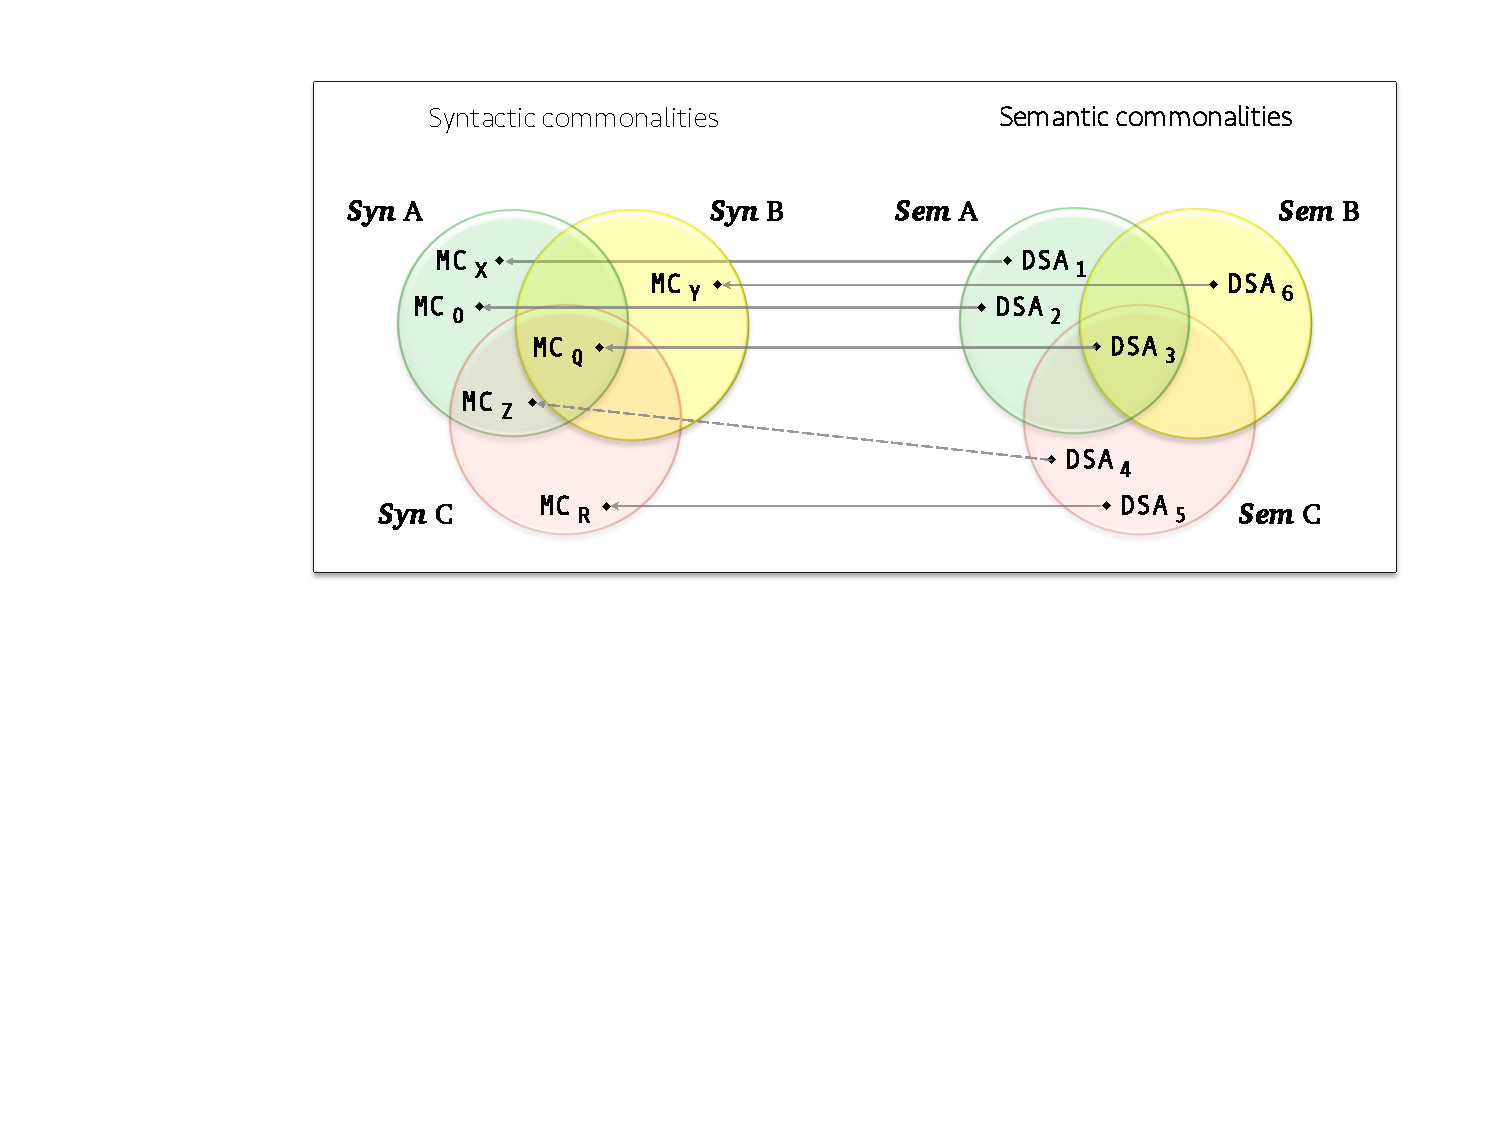
\includegraphics[width=1\linewidth]{images/domains-fig.pdf}
\caption{Commonalities between domains and potential reuse}
\label{fig:domains}
\end{figure}

Commonalities can be found between two ore more DSLs of the input set. That is, we can find metaclasses and domain specific actions that are shared by more than two DSLs. Hence, intersections should be searched among all the possible combinations of the DSLs in the input set. Once those functions are defined and implemented, the second phase is to use them in order to find the intersections among the DSLs of the input set. 

\vspace{-3mm}
\subsubsection{Semantical variability:} Note that the fact that two metaclasses are shared does not imply that all their domain specific actions are the same. In that figure, we see this in the case of MMz. This metaclass is shared by the DSLs A and C but, in each DSL the semantics is different since each of them implement a different DSA for the metaclass. We refer to that phenomenon as \textit{semantical variability}. There are two constructs that share the syntax but that differ in their semantics. In such case, there is potential reuse at the level of the syntax since the metaclass can be defined once and reused in the DSLs but the semantics should be defined differently for each DSLs. 

%there are three DSLs DSLs that are totally independent. That means that they do not share any of their language constructs, and consequently, there is not potential reuse between them. Differently, the two DSLs shown at the right of the figure have overlapping domains. That means that there are a subset of language that are \large\textbf{``equal'' }\normalsize in both DSLs. Note that if two language constructs are the same, we can assume that their specifications are equal and can be reused instead of being replicated.




%Moreover, there are set of DSLs for which the domains can be hierarchically organized \cite[p. 60-61]{voelter:2013}.

%\subsection{Equivalence between language constructs}

%So far, we have based the notion of potential reuse in DSLs on the commonalities existing in a set of DSLs. Nevertheless, this assumption supposes that we are able to compare two language constructs in order to know if they are equivalent. So, now we need to define this \textit{equivalence} relationship. In particular, the comparison of two language constructs relies on two dimensions: (1) comparison of the meta-classes in the abstract syntax; and (2) comparison of the domain-specific actions in the semantics.


%\section{Motivation}
\label{sec:motivation}

Consider a team of language designers working on the construction of the DSLs for state machines presented in section \ref{sec:background}. During that process, language designers implement the language constructs typically required for expressing finite state machines: states, transitions, events, and so on. In addition, the DSL is intended to provide a constraints language that allows final users to express guards on the transitions. Moreover, the DSL also provides an expressions language that allows to specify actions on the states of the state machine. This expressions language offers classical capabilities such as arithmetic operations, variables management, and imperative procedures. 

After being released their DSL for state machines, the language development team is required again. This time the objective is to build a DSL for manipulating the traditional Logo turtle which is often used in elementary schools for teaching the first foundations of programming \cite{Olson:1987}. Certainly, the new DSL is essentially different from the DSL for state machines. Instead of states and transitions, Logo offers some primitives (such as \texttt{Forward}, \texttt{Backward}, \texttt{Left}, and \texttt{Right}) to move a character (i.e., the turtle) within a bounded canvas. However, Logo also requires an expressions language in order to specify complex movements. For example, final users may write instructions such as: \texttt{forward (x + 2)} where \texttt{x} is a variable.

At this point, language designers face the question of how to reuse the expressions language they already defined for the state machines language. As illustrated in Figure \ref{fig:cloning}, the typical solution to this type of situations is to replicate the code in a second DSL. Language designers usually copy/paste the segment of the specification that they can reuse. As a result, we have many clones that are expensive to maintain. Naturally, this situation is repeated each time that there is a new DSL to build. This fact is illustrated in the Figure \ref{fig:cloning} by introducing a third DSL for expressing flowcharts. In this case, the new DSL requires both, expressions and constraints languages. 

\begin{figure}
\centering
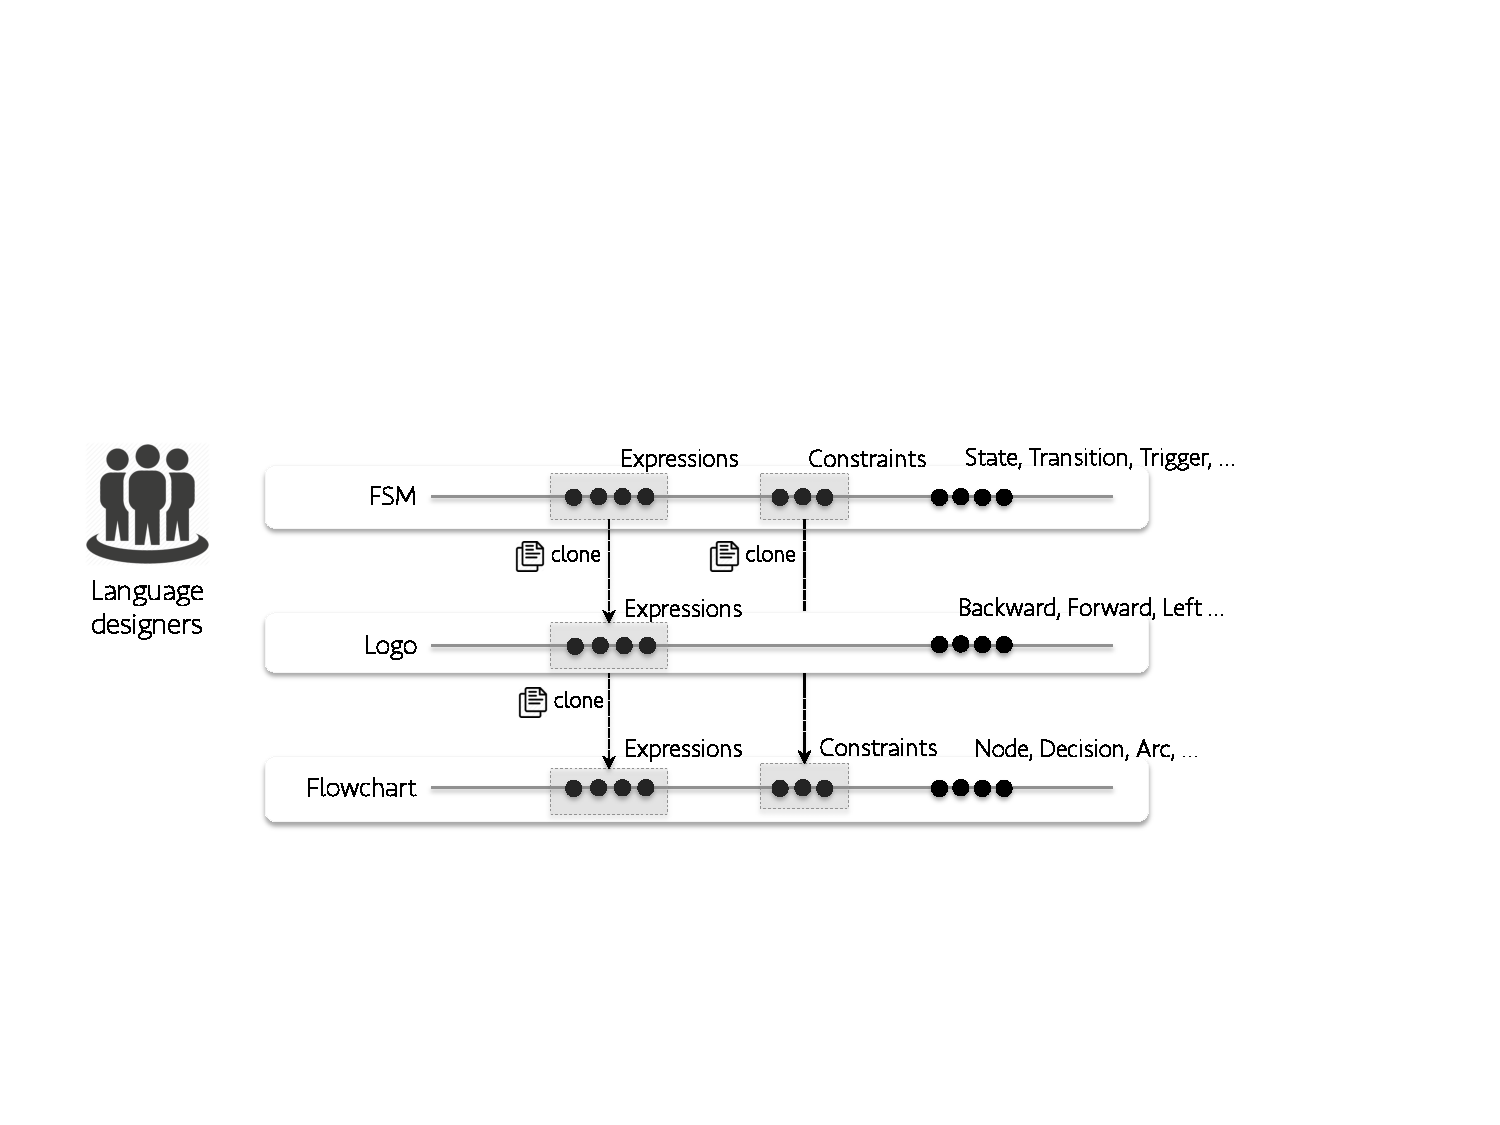
\includegraphics[width=1\linewidth]{images/cloning.pdf}
\caption{Cloning in DSLs development process}
\label{fig:cloning}
\end{figure}

%As a matter of fact, these DSLs are essentially different. Each of them is focus on a particular domain and offers different language constructs. However, there are syntactic and semantic commonalities that are illustrated in Figure \ref{fig:domains}. All the thee DSLs offer some expressions for modifying variables. In the case of FSM these actions are needed the specification of the actions in the states; in the case of Logo expressions are needed to specity the movement and rotation parameters; and in the case of flowchart expressions are needed to specify the body of actions. In addition, both FSM and Flowchart rely on a constraints language. The former for expressing guards in the transitions and the later for expressing guards of the decisions.

\textbf{Overlapping in DSLs and potential reuse:} The aforementioned phenomenon was previously observed by V\"oelter et al \cite[p. 60-61]{voelter:2013}. In fact, that study demonstrates that although many of the existing DSLs are completely different and tackle independent domains; there are related DSLs with overlapping domains. That is, they share certain language constructs i.e., they have \textbf{commonalities} between them. Figure \ref{fig:shape} illustrates this observation for the case of our illustrating scenario and by using two Venn diagrams to represent both syntax and semantic overlapping. Syntactic and semantic overlapping is represented as intersections between the corresponding sets. To this end, we designed an algorithm that is able to compute the all overlapping among the syntax of the DSLs in the input set. 

\begin{figure}
\centering
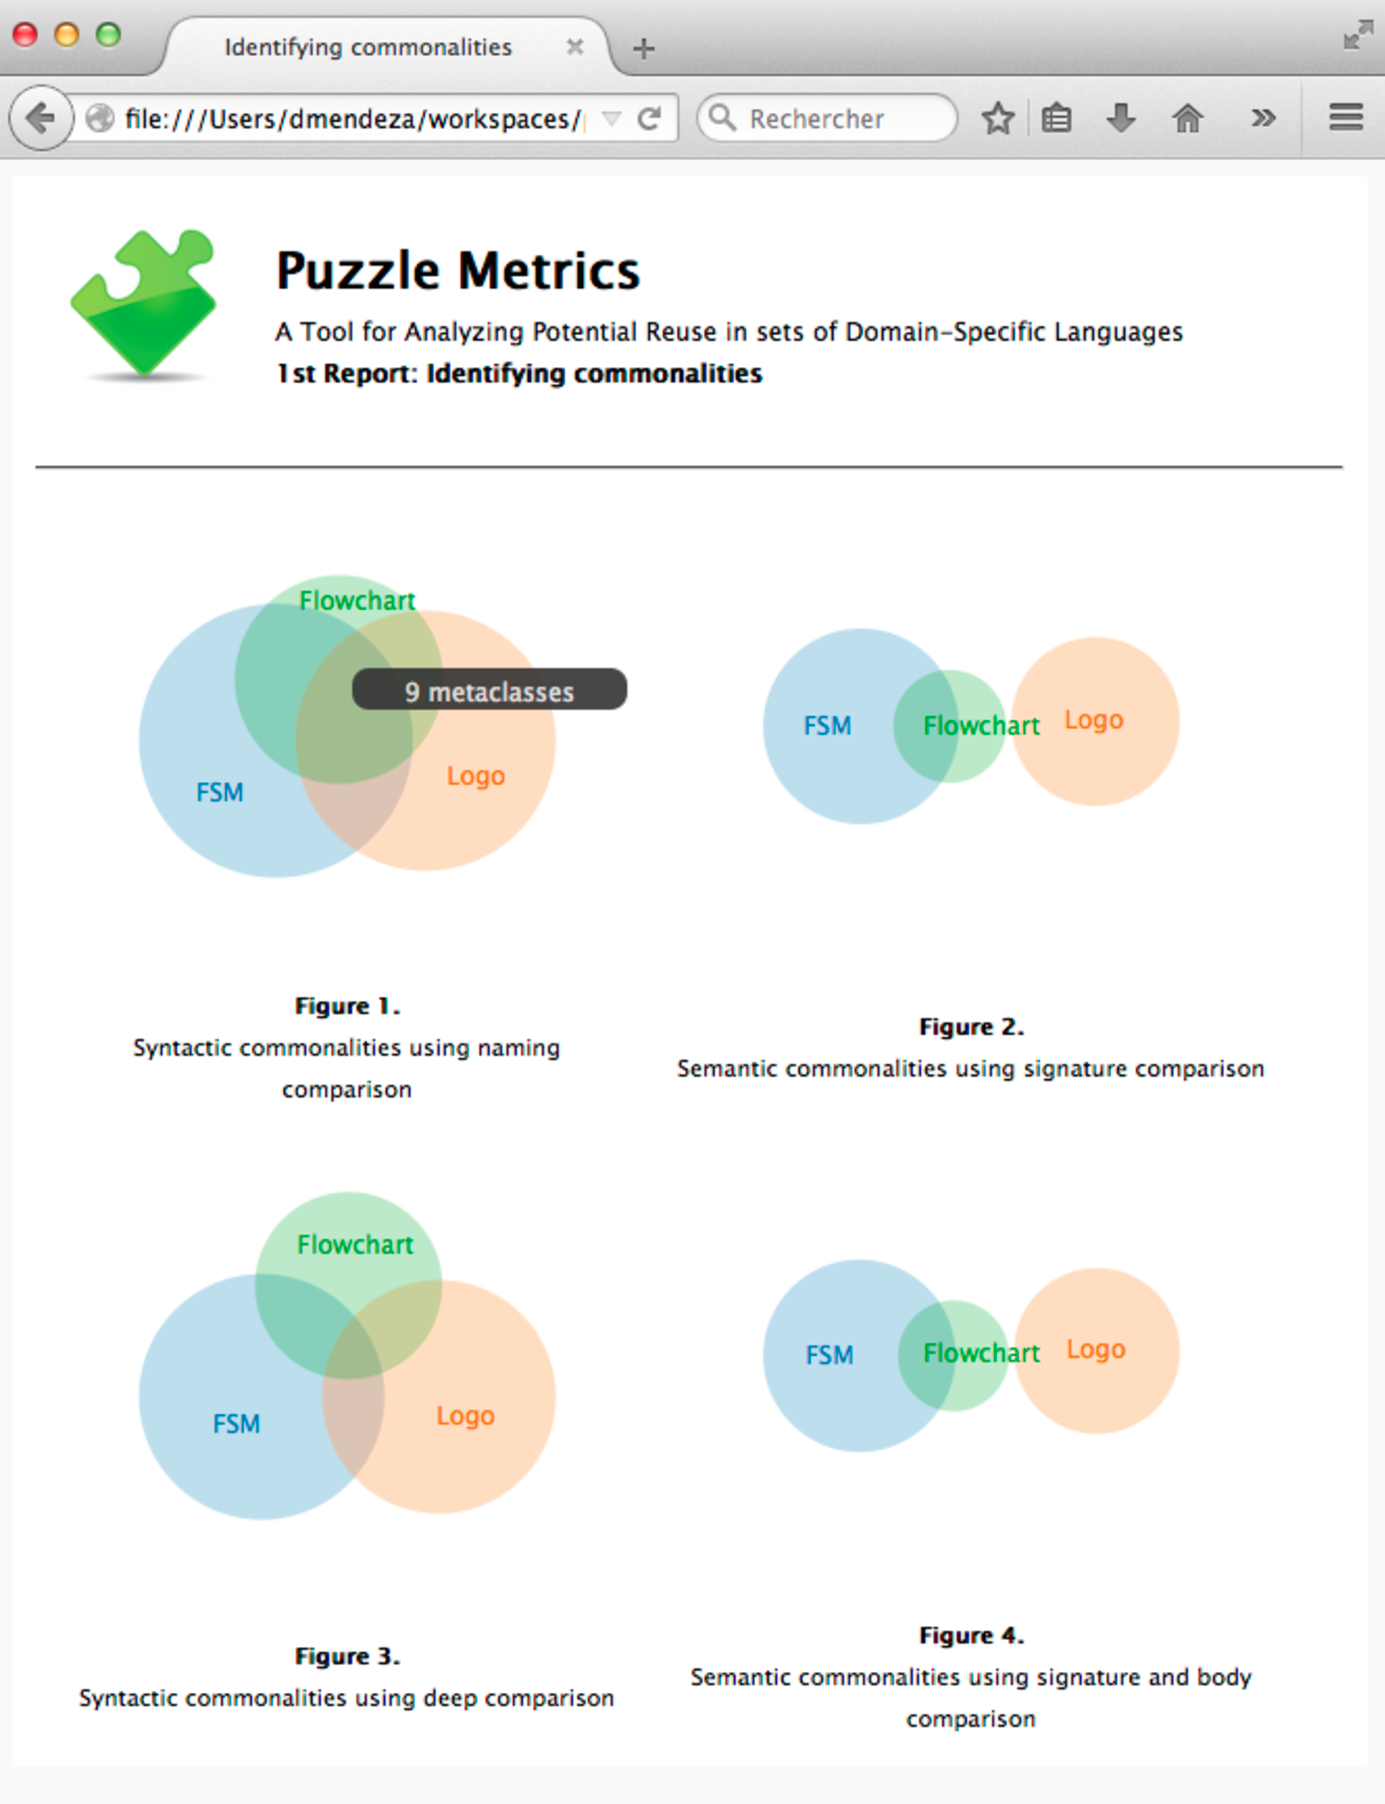
\includegraphics[width=1\linewidth]{images/domains-inaction.pdf}
\caption{Visualizing syntactic and semantic commonalities}
\label{fig:shape}
\end{figure}

If a set of DSLs have some overlapping and they are specified in the same technological space and using compatible language workbenches, then there is \textbf{potential reuse} since the specification of those shared constructs can be specified once and reused in the two DSLs \cite[p. 60-61]{voelter:2013}. For the technological space discussed in this paper, syntactic commonalities appear where DSLs share some metaclasses and semantic commonalities appear where DSLs share some domain-specific actions.

%Figure \ref{fig:domains} illustrates the phenomenon in our illustrating scenario. Note that each DSL is specified in terms of a set of metaclasses (top of the figure), and a set of aspects (bottom of the figure) that weave some domain-specific actions to the metaclasses. In the case of this example, the semantics of the metaclasses expression and constraints are also shared. That means that the semantics are the same. 

It is worth to mention that the fact that two metaclasses are shared does not imply that all their domain specific actions are the same. We refer to that phenomenon as \textbf{semantical variability}. There are two constructs that share the syntax but that differ in their semantics. In such case, there is potential reuse at the level of the syntax since the metaclass can be defined once and reused in the DSLs but the semantics should be defined differently for each DSLs. 

%\begin{figure}
%\centering
%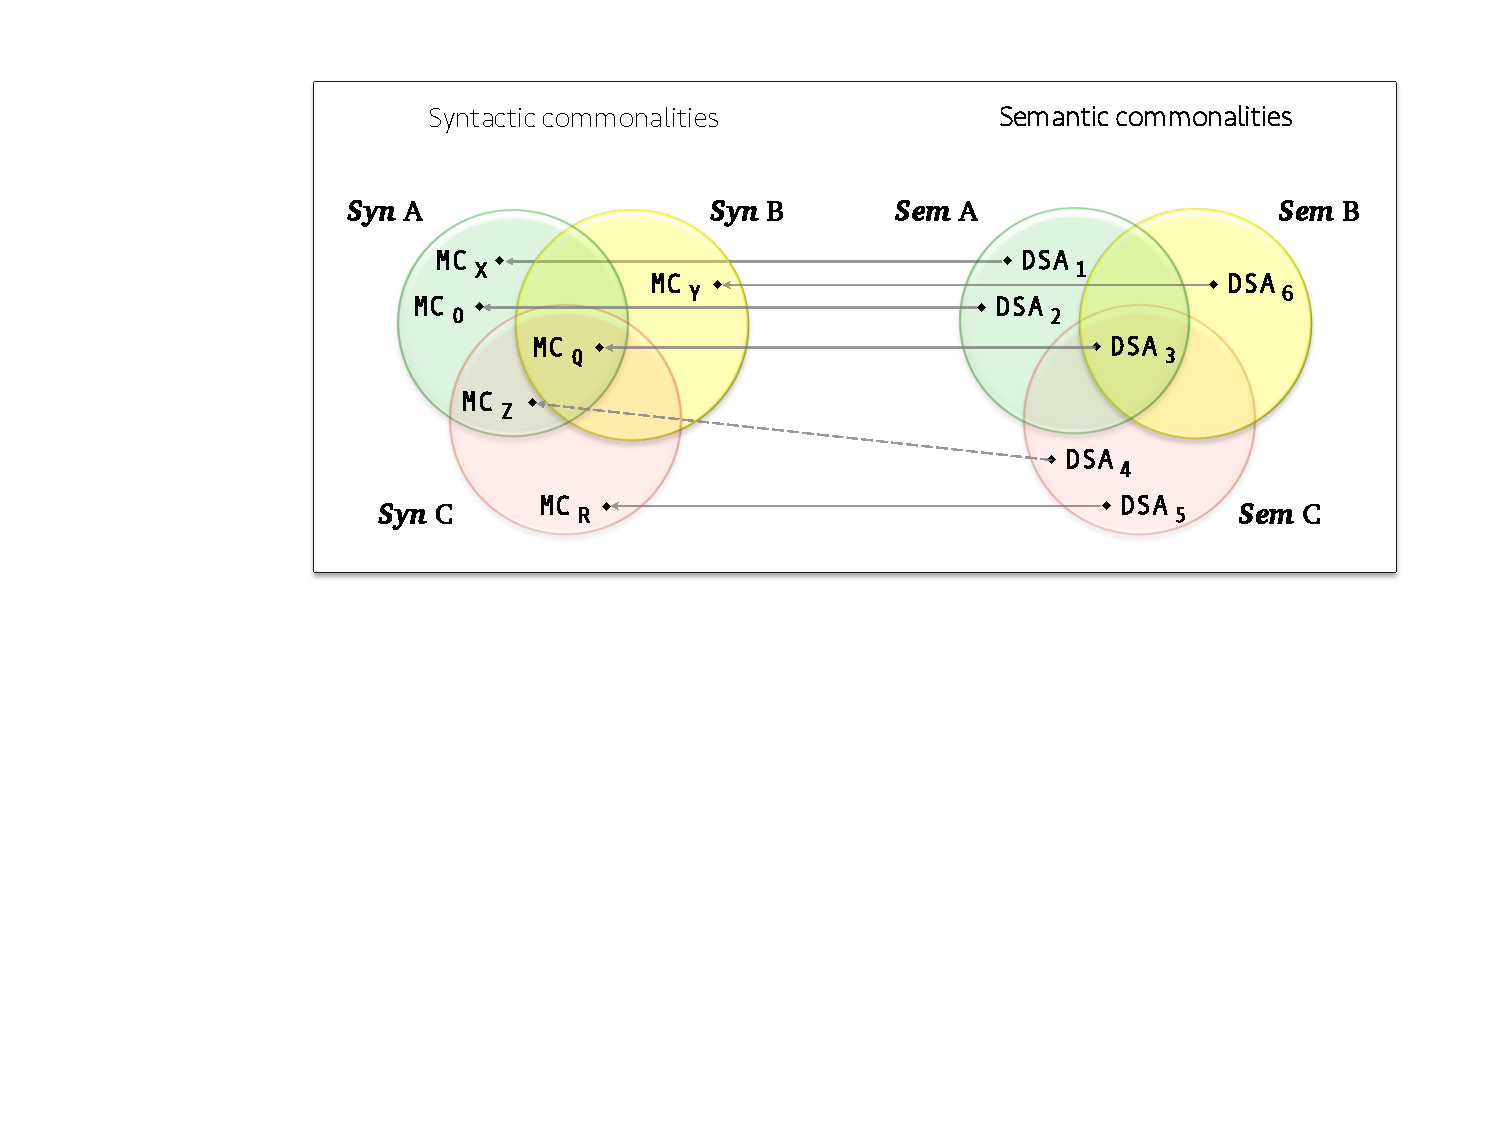
\includegraphics[width=1\linewidth]{images/domains-fig.pdf}
%\caption{Commonalities between domains and potential reuse}
%\label{fig:domains}
%\end{figure}

%Commonalities can be found between two ore more DSLs of the input set. That is, we can find metaclasses and domain specific actions that are shared by more than two DSLs. Hence, intersections should be searched among all the possible combinations of the DSLs in the input set. Once those functions are defined and implemented, the second phase is to use them in order to find the intersections among the DSLs of the input set. 



%there are three DSLs DSLs that are totally independent. That means that they do not share any of their language constructs, and consequently, there is not potential reuse between them. Differently, the two DSLs shown at the right of the figure have overlapping domains. That means that there are a subset of language that are \large\textbf{``equal'' }\normalsize in both DSLs. Note that if two language constructs are the same, we can assume that their specifications are equal and can be reused instead of being replicated.




%Moreover, there are set of DSLs for which the domains can be hierarchically organized \cite[p. 60-61]{voelter:2013}.

%\subsection{Equivalence between language constructs}

%So far, we have based the notion of potential reuse in DSLs on the commonalities existing in a set of DSLs. Nevertheless, this assumption supposes that we are able to compare two language constructs in order to know if they are equivalent. So, now we need to define this \textit{equivalence} relationship. In particular, the comparison of two language constructs relies on two dimensions: (1) comparison of the meta-classes in the abstract syntax; and (2) comparison of the domain-specific actions in the semantics.


\section{Proposed approach}
\label{sec:apprach}

Our objective is to extract a catalog of reusable language modules from a given set of DSLs (that we refer to as the \textit{input set}). To this end, we propose an approach based on the aforementioned notions of overlapping and potential reuse. Concretely, in our approach we first identify syntactic and semantic overlapping among the DSLs of the input set. Then, we cut such overlapping in order to break-down the DSLs in reusable language modules. Those language modules are encapsulated in such a way that they can be later composed among them to obtain complete DSLs. The overall strategy is illustrated in Figure \ref{fig:breakingdown}. This section is dedicated to explain it in detail.

\begin{figure}
\centering
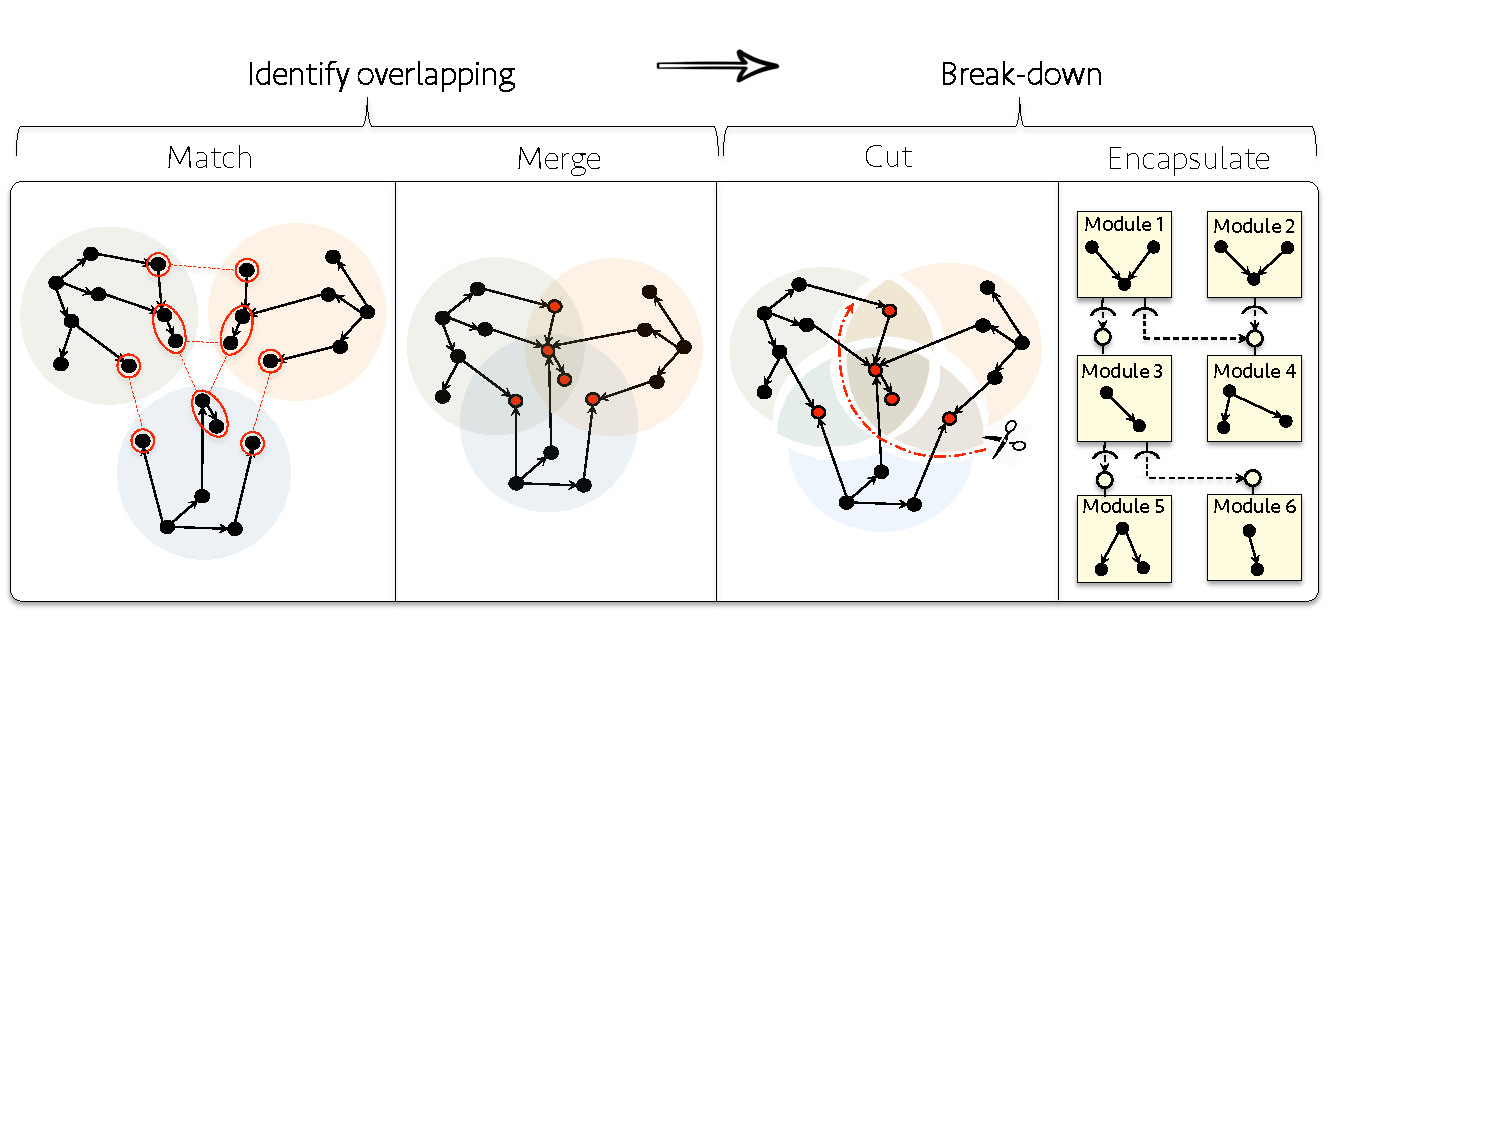
\includegraphics[width=1\linewidth]{images/breakdown.pdf}
\caption{Breaking down the input set by cutting overlapping}
\label{fig:breakingdown}
\end{figure}

\subsection{Identifying overlapping: \textit{match} and \textit{merge}}
\label{sec:identifyingoverlapping}

Our strategy to identify \textbf{syntactic overlapping} is based on the fact that a metamodel can be viewed as a direct graph $DAG=<V,A>$ where the vertex $V$ represent metaclasses and the arcs $A$ represent references between metaclasses. Since each DSL of the input set has a metamodel that represents its syntax, syntactic overlapping can be detected by identifying replicated vertex among the corresponding graphs, and organize them in the form of a Venn diagram as illustrated in the two first steps shown in Figure \ref{fig:breakingdown}.

Following this principle, we identify syntactic overlapping by means of a twofold algorithm. First, we perform a matching process that receives a set of graphs (one for each metamodel) and returns the collection of vertex referencing metaclasses that are \textit{identical}. Second, we merge the matched vertex, thus removing replications. In order to create the intersections, we store the information about what are the DSLs where the corresponding metaclass is defined.

Once matched vertex are merged, we analyze the domain specific actions associated to the corresponding metaclasses. Particularly, for each set of identical metaclasses we check if the domain-specific actions are equal as well. If so, we also have \textbf{semantic overlapping} and then we merge the domain-specific actions as well because they are replicated code. Otherwise, we create different clusters of domain-specific actions, one for each metaclass, thus establishing a \textbf{semantic variation point}. In other words, we create two different implementations of the semantics of the same metaclass.

%\begin{equation}
%  Venn_{syn} : set(MM) \rightarrow set(<set(MM),set(MC)>)
%\end{equation}

%\begin{equation}
%  Venn_{syn}(mms) = \{<x,y> \mid x \in \mathcal{P}(mms), y = I_{syn}(x)\}
%\end{equation}

%Note that our algorithm relies on a function $I_{syn}$ that computes the intersection existing withing a given set of metamodels. It can be formalized as follows:

%\begin{equation}
%  I_{syn} : set(MM) \rightarrow set(MC)
%\end{equation}
%\vspace{-2mm}
%\begin{equation}
%  I_{syn}(mms) = \bigcap _{i=0}^{|mms|}mms_i
%\end{equation}

%Similarly, our algorithm for detecting \textbf{semantic intersections} can be described as a function that receives a set of aspects (one for each DSL of the input set) and returns a set of tuples containing all the intersections among these aspects. 

%\begin{equation}
%  Venn_{sem} : set(A) \rightarrow set(<set(A),set(DSA)>)
%\end{equation}

%\begin{equation}
%  Venn_{syn}(mms) = \{<x,y> \mid x \in \mathcal{P}(mms), y = I_{sem}(x)\}
%\end{equation}
%\vspace{2mm}

%This time, the algorithm for semantic commonalities relies on a function $I_{sem}$ that computes the intersection existing withing a given set of aspects. It can be formalized as follows:

%\begin{equation}
%  I_{sem} : set(A) \rightarrow set(DSA)
%\end{equation}
%\vspace{-2mm}
%\begin{equation}
%  I_{sem}(dsas) = \bigcap _{i=0}^{|dsas|}dsas_i
%\end{equation}

It is worth noting that detection of both syntactic and semantic overlapping relies on comparison of metaclasses and domain-specific actions respectively. At this point we need to clearly define such notion of equality that, as a matter of fact, is quite important to avoid alterations on the DSLs after the extraction of reusable language modules.

\vspace{-3mm}
\subsubsection{Comparison of metaclasses:} An operator for metaclasses comparison can be specified as follows: 

\begin{equation}
  \doteq~: MC \times MC \rightarrow bool
\end{equation}

To implement such operator, one can intuitively think that a first approach to compare meta-classes is by comparing their names. Certainly, this approach results quite useful and it is quite probable that, we can find potential reuse. For example, one can expect that in a set of DSLs for finite state machines DSL, the construct \texttt{Transition} can be considered as a commonality.

Unfortunately, comparison of metaclasses by using only their names might have some problems. There are cases in which two meta-classes with the same name are not exactly the same since they do not represent the same domain concept or because there are domains that use similar vocabulary. For instance, whereas in many cases the transitions of a state machine are only specified in terms of triggers and constraints, there are certain DSLs for state machines that allow to annotate transitions are annotated with time flags \cite{Graf:2007}.

In such cases, feasibility of potential reuse is not clear because the involved metaclasses offer different functionalities. Hence, a more restrictive operator should be considered. An approach that certainly helps is to compare metaclasses not only by their names but also by their attributes and references. Although this strategy can be quite restrictive, it guarantees that the detected reuse opportunities correspond to exact code clones so they can be extracted as reusable modules without any risk of altering the behavior of the DSLs. In our approach we use the later strategy. Nevertheless, we consider that certain flexibility might be to define those operators. We provide an extensible approach where other operators (such as the surveyed in \cite{Lafi:2011}) can be easily incorporated.

%\vspace{-1mm}
%\begin{equation}
%\begin{split}
%  MC_{A} \doteq MC_{B} &= true \implies \\
%   & MC_{A}.name = MC_{B}.name
% \end{split}
%\end{equation}

%\begin{equation}
%  \doteqdot~: MC \times MC \rightarrow bool
%\end{equation}
%\vspace{-1mm}
%\begin{equation}
%\begin{split}
%  MC_{A} \doteqdot MC_{B} &= true \implies \\
%   & MC_{A}.name = MC_{B}.name ~ \wedge \\
%   & \forall a_1 \in MC_{A}.attr \mid (\exists a_2 \in MC_{B}.attr \mid a_1 = a_2) ~ \wedge \\
%   & \forall r_1 \in MC_{A}.refs \mid (\exists r_2 \in MC_{B}.refs \mid r_1 = r_2)
%  \end{split}
%\end{equation}

\vspace{-3mm}
\subsubsection{Comparison of domain-specific actions:} In turn, the operator for comparison of domain-specific actions can be specified as follows:

\begin{equation}
  \circeq~: DSA \times DSA \rightarrow bool
\end{equation}

Like methods in Java,domain specific actions have a signature that specifies its contract (i.e., return type, visibility, parameters, name, and so on), and a body where the behavior is actually implemented. In that sense, the implementation of a comparison operator for domain-specific actions can be performed by checking if their signatures are equal. This approach is practical and also reflects potential reuse; one might think that the probability that two domain-specific actions with the same signatures are the same is elevated.

However, during the conduction of this research we realized that there are cases in which signatures comparison is not enough. Two domain-specific actions defined in different DSLs can perform different computations even if they have the same signatures. For example, we can found semantic variation points in the implementation of DSLs for state machines where the domain-specific actions are implemented differently although their signatures are the same. As a result, we only guarantee potential reuse where we compare also the bodies of the domain-specific actions. 

Note that such comparison can be arbitrary difficult. Indeed, if we try to compare  the behavior of the domain-specific actions we will have to deal with the semantic equivalence problem that, indeed, is known to be undecidable \cite{Lucanu:2013}. To deal with this issue, we compare the body of domain-specific actions by in terms of its abstract syntax tree as proposed by Biegel et al \cite{Biegel:2010}. This strategy guarantees that semantic overlapping correspond to exact clones. Again, our approach can be extended to support other comparison operators for domain-specific actions. 

%\vspace{-1mm}
%\begin{equation}
%\begin{split}
%  DSA_{A} & \circeq DSA_{B} = true \implies \\
%   & DSA_{A}.name = DSA_{B}.name ~ \wedge \\
%   & DSA_{A}.returnType = DSA_{B}.returnType ~ \wedge \\
%   & DSA_{A}.visibility = DSA_{B}.visibility ~ \wedge \\
%   & \forall p_1 \in DSA_{A}.params \mid (\exists p_2 \in %DSA_{B}.params \mid p_1 = p_2)
% \end{split}
%\end{equation}

%\begin{equation}
%  \triangleq~: DSA \times DSA \rightarrow bool
%\end{equation}
%\vspace{-1mm}
%\begin{equation}
%\begin{split}
%  DSA_{A} & \circeq DSA_{B} = true \implies \\
%   & DSA_{A}.name = DSA_{B}.name ~ \wedge \\
%   & DSA_{A}.returnType = DSA_{B}.returnType ~ \wedge \\
%   & DSA_{A}.visibility = DSA_{B}.visibility ~ \wedge \\
%   & \forall p_1 \in DSA_{A}.params \mid (\exists p_2 \in DSA_{B}.params \mid p_1 = p_2)  ~ \wedge \\
%   & DSA_{A} \circeq DSA_{B} ~ \wedge \\
%   & DSA_{A}.AST = DSA_{B}.AST
% \end{split}
%\end{equation}


%It is worth nothing that there is this phenomenon of \textit{semantical variability}. A necessary condition to decide whether two language constructs are equivalent is that both, the metaclass and the associated domain-specific actions are equivalent. This condition guarantees that the specification is the same not only at the level of the abstract syntax but also at the level of the semantics. However, there is a phenomenon in the literature that corresponds to semantical variability \cite{Cengarle:2009}. There is semantical variability when there there are two constructs that have the same abstract syntax (i.e., their metaclasses are equal) but that differ in the domain-specific actions. This case is of interest for us because even in the presence of semantical variability we can have some potential reuse. If the metaclasses of two constructs are the same we can reuse them even if their domain-specific actions are different. 

%\vspace{-2mm}
%\subsubsection{Visualizing semantical variability:} Note that the phenomenon of semantical variability is evident in the example presented. Where there are syntactic commonalities between DSLs Logo and FSM, there are not semantic commonalities. As an additional feature of our approach, we provide a visualization of the semantical variability phenomenon. The idea is that language designers can see what are the variations in the domain specific actions.
%\todo[inline]{Usa el ejemplo para ejemplificar}

\subsection{Breaking down the input set: \textit{cut} and \textit{encapsulate}}

After being identified overlapping among the DSLs in the input set, we extract a set of reusable language modules. To this end, we adopt the idea presented by V\"oelter et al \cite[p. 60-61]{voelter:2013}: we break-down the overlapping by creating one language module for each different intersection as illustrated in the third step of Figure \ref{fig:breakingdown}. The reasoning to this solution is quite simple: by definition, an intersection is a set of language constructs that are shared by two or more DSLs. If we extract those language constructs in separated language modules, the language module can be defined once and reused by all the DSLs that require it. So, we can consider that the extracted language module is reusable. 

In our approach, we implemented this separation of overlapping as a graph partitioning algorithm. The algorithm receives the graph(s) obtained from the merging process and returns a set of node clusters: one cluster for each intersection of the Venn diagram. Arcs defined between nodes in different clusters can be considered as cross-cutting dependencies between clusters. Then, we encapsulate each nodes cluster in the form of language modules. Each module contains a metamodel, a set of domain-specific actions, and a set of dependences towards other language modules. 

Dependencies between language modules are supported by means of the classical required and provided roles in components-based software development. There is a \textit{requiring module} that uses some constructs provided by a \textit{providing module}. The requiring module has a dependency relationship towards the providing one that, in the small, is materialized by the fact that some of the classes of the requiring module have references (simple references, containment references, or inheritances) to some constructs of the providing one. In order to avoid direct references between modules, we introduce the notion of interfaces for dealing with modules' dependencies. The requiring language has a \textit{required interface} whereas the providing one has the \textit{provided interface}. A required interface contains the set of constructs required by the requiring module which are supposed to be replaced by actual construct provided by other module(s) (see Figure \ref{fig:approaches-interfaces}).

We use \textit{model types} \cite{Steel:2007} to express both required and provided interfaces. A module can have some references to the constructs declared in its required interface. In turn, the relationship between a module and its provided interface is \textit{implements} (deeply explained in \cite{Degueule:2015}). A module implements the functionality exposed in its model type. If the required interface is a subtype of the provided interface, then the provided interface fulfills the requirements declared in a required interface. 

\begin{figure}
\centering
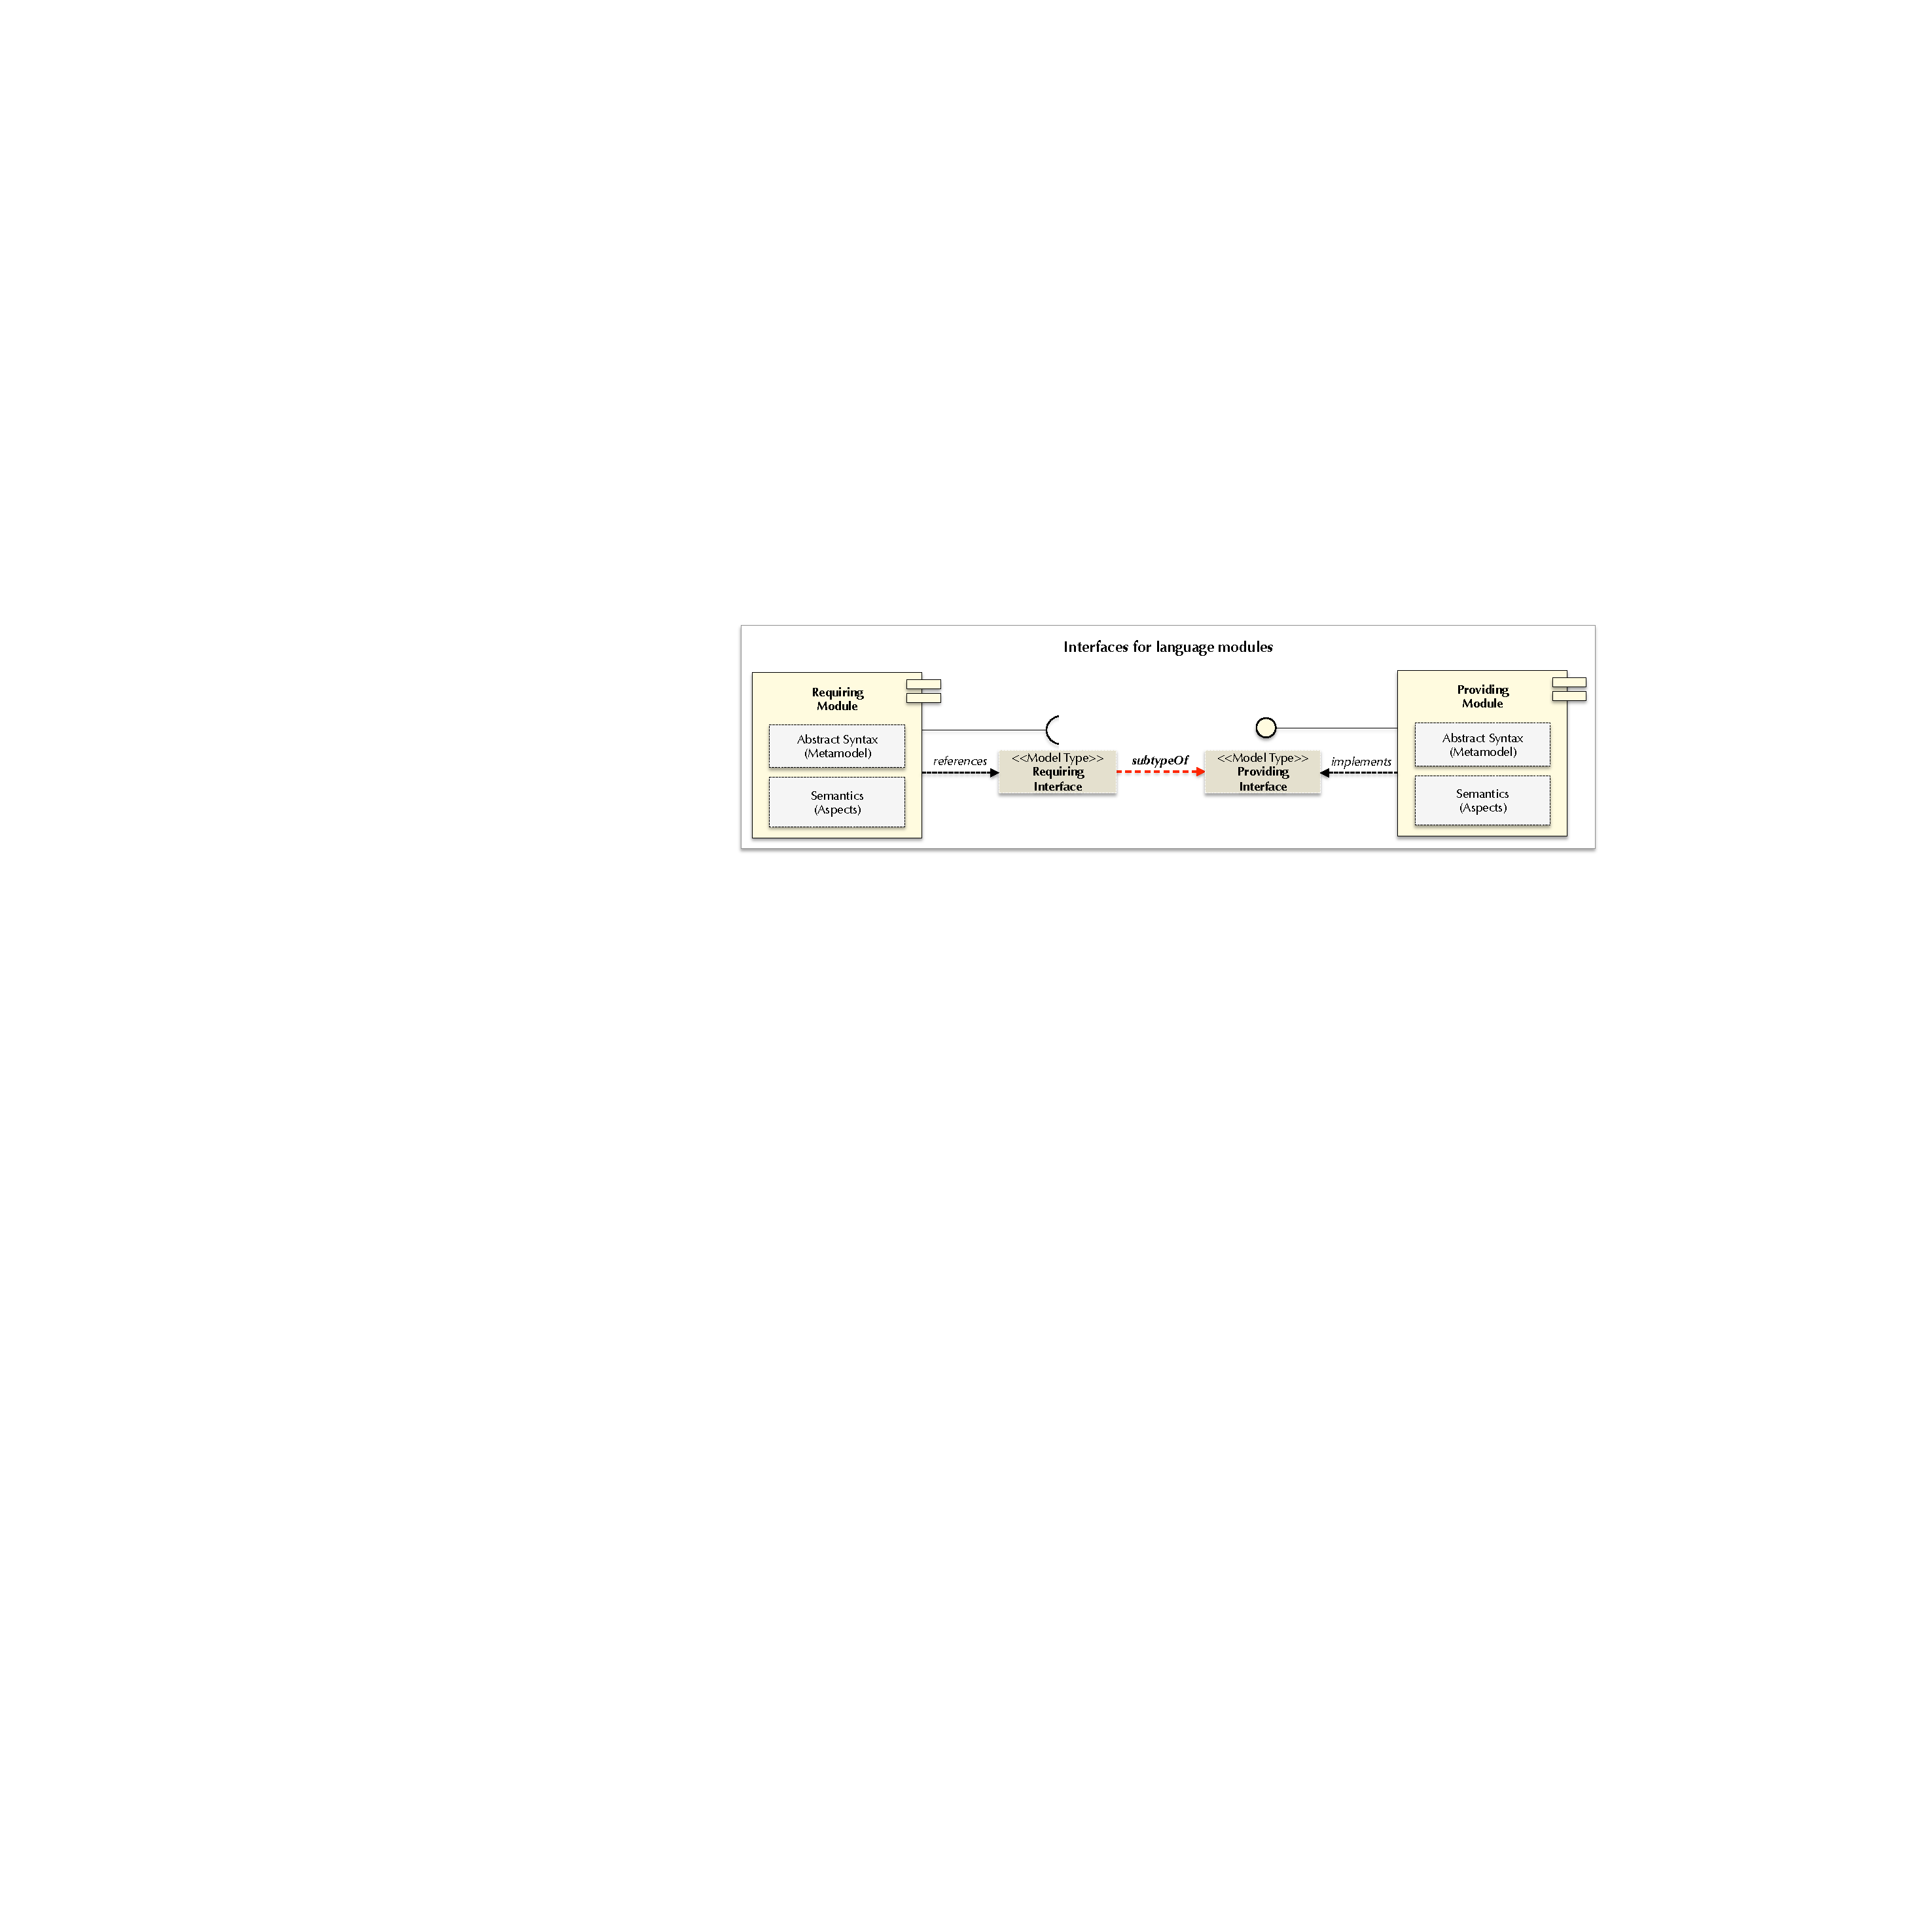
\includegraphics[width=1\linewidth]{images/approach-interfaces.pdf}
\caption{Interfaces for language modules}
\label{fig:approaches-interfaces}
\end{figure}
\vspace{-3mm}

%\section{Evaluation}
\label{sec:validation}

In this section we present the validation of our approach. As aforementioned, this validation is twofold. On one hand, we demonstrate that our approach is correct. To do so, we take use a case study that is well documented in \cite{Crane:2007} and where we exactly know the commonalities existing among the input set. We execute our approach and we compare the results while expecting that the input of our tool matches with the commonalities we know. It is important to mention that this case study corresponds to a real problematic in the industry. Concretely, it is one of the motivations of the VaryMDE\footnote{\url{http://varymde.gforge.inria.fr/}} project which is a collaboration between Thales Research \& Technology, and INRIA.  

The second part of the evaluation corresponds to demonstrate that our approach is relevant. We demonstrate, with empirical data, that the phenomenon of syntactic and semantic commonalities is currently appearing in real DSLs and, so, there is an important amount of potential reuse in the wild and our approach can be actually useful. 

\subsection{Evaluating \textit{correctness}: The state machines case study}

The case study is composed of three different DSLs for expressing state machines:  UML state diagrams \cite{UML:2011}, Rhapsody \cite{Harel:2004}, and Harel's state charts \cite{Harel:1996}. Because the three DSLs are intended to express the same formalism, they have commonalities. For example, all of them provide basic concepts such as \texttt{StateMachine}, \texttt{State}, \texttt{Transition}, or \texttt{Trigger}. However, not all those DSLs are equal. In fact, they have some syntactic and semantic differences which are well documented in the Crane's article \cite{Crane:2007}. To validate our approach we implemented these three DSLs while strictly following that documentation. Thus, we obtained a set of DSLs to test our tool and we know in advance the results that the tool should provide. We use that as an oracle to test our approach. 

\begin{figure}
\centering
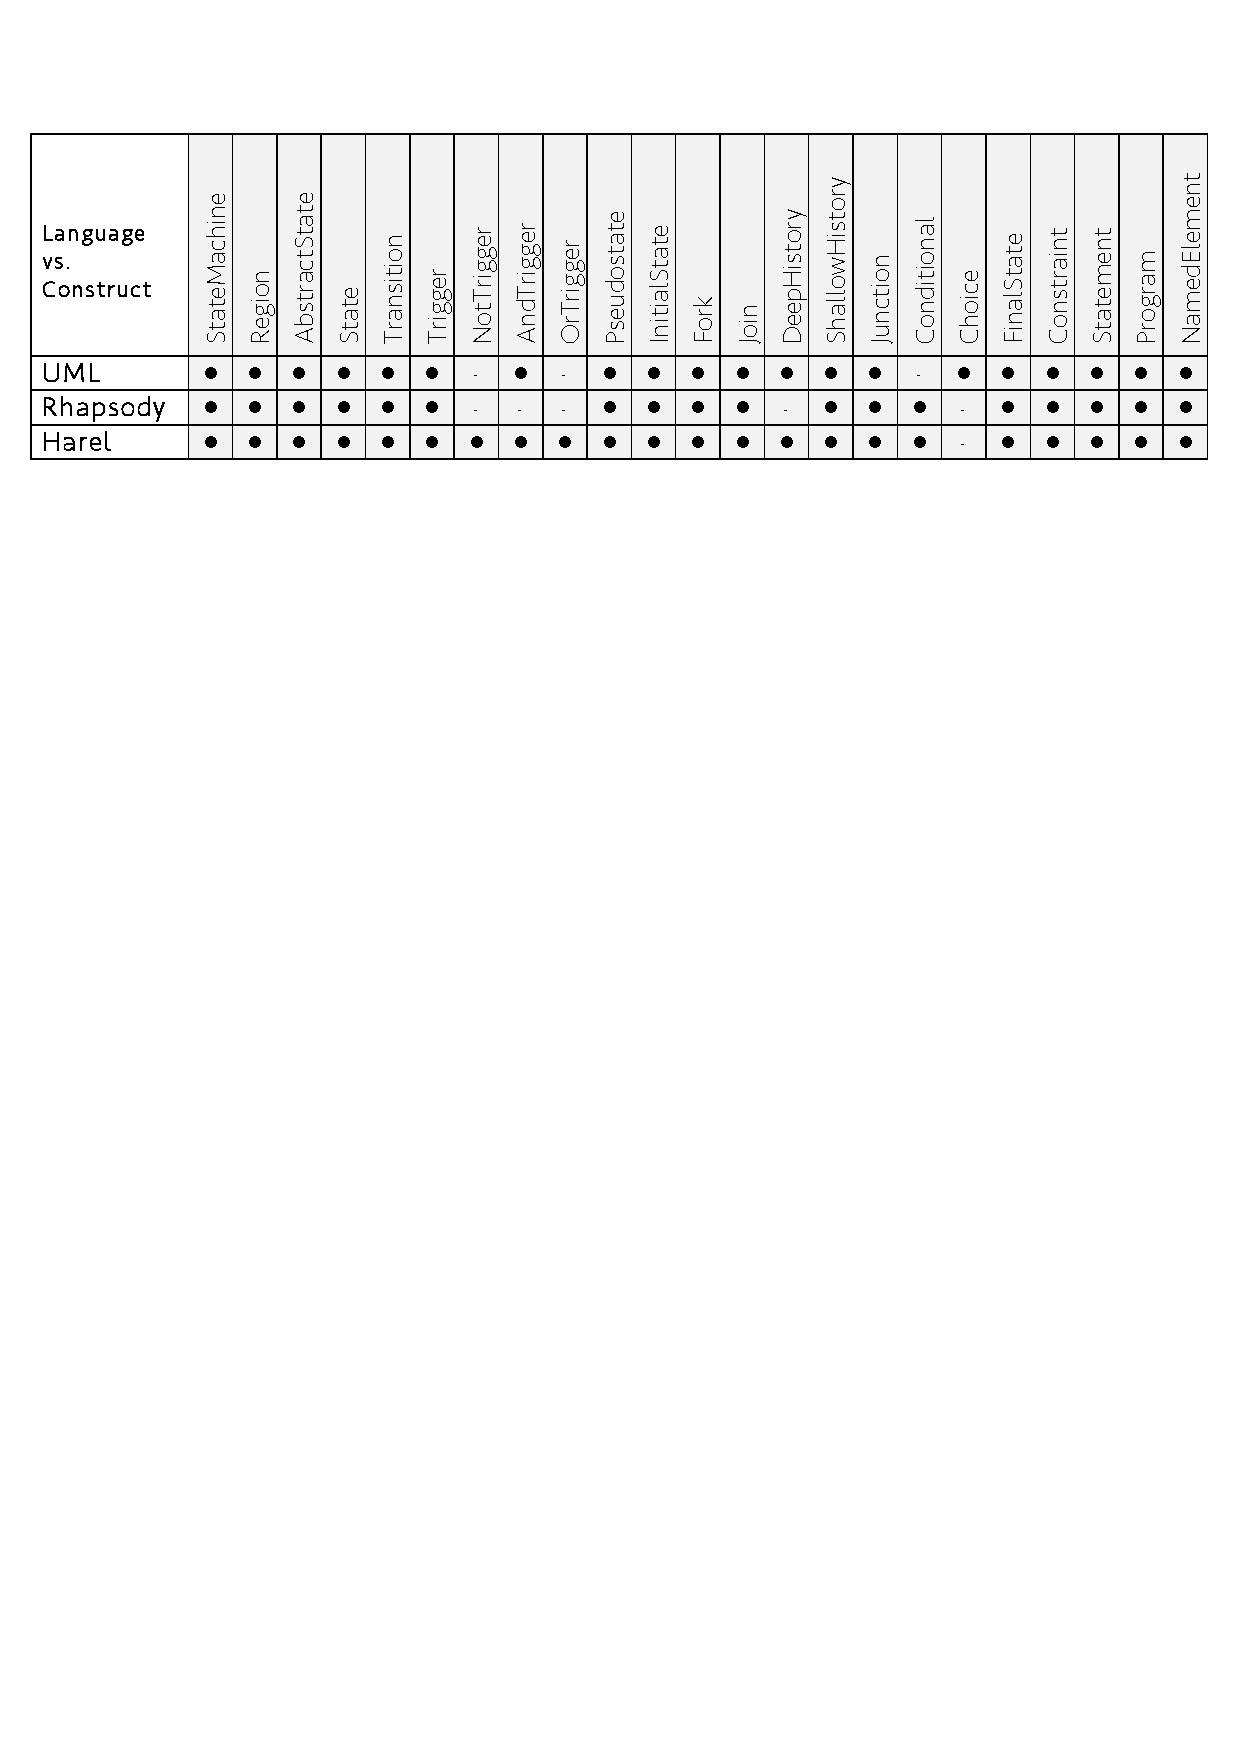
\includegraphics[width=1\linewidth]{images/oracle.pdf}
\caption{Oracle for evaluation of correctness}
\label{fig:oracle}
\end{figure}

\subsubsection{Oracle.} Figure \ref{fig:oracle} shows a table with the constructs contained by each DSL in the case study. Note that not all the DSLs have exactly the same constructs. The main differences are in the support for types of triggers. Whereas Rhapsody only supports simple triggers. Harel's state charts and UML provide support composing triggers. In particular, in Harel's state charts triggers can be composed by using \texttt{AND}, \texttt{OR}, and \texttt{NOT} operators. In turn, in UML triggers can be composed by using only the \texttt{AND} operator. Another difference between the DSL of our case study corresponds to the different support for pseudostates. Whereas there are pseudostates that are supported by all the DSLs (\texttt{Fork}, \texttt{Join}, \texttt{ShallowHistory}, and \texttt{Junction}); there are certain psueudostates such as \texttt{DeepHistory}, \texttt{Conditional}, or \texttt{Choice} that are not supported in all of the DSLs.

In summary, there are: 17 language constructs that are shared by all the DSLs; 1 construct that is exclusive of UML, 2 constructs that are exclusive of Harel's state charts; 2 constructs shared by UML and Harel's state charts; and 1 construct shared by Harel's state charts and Rhapsody. 

\vspace{-2mm}
\subsubsection{Results.} Figure \ref{fig:puzzle-overlapping} shows the results of the first part of the analysis. It presents the Venn diagram produced for the case study of the state machines. Note that the numbers correspond to our oracle demonstrating that our approach is correct. Due to lack of space, we do not present the semantic results. However, in a later section we present a tool demonstration that shows the complete functionality of our tool.

\begin{figure}
\centering
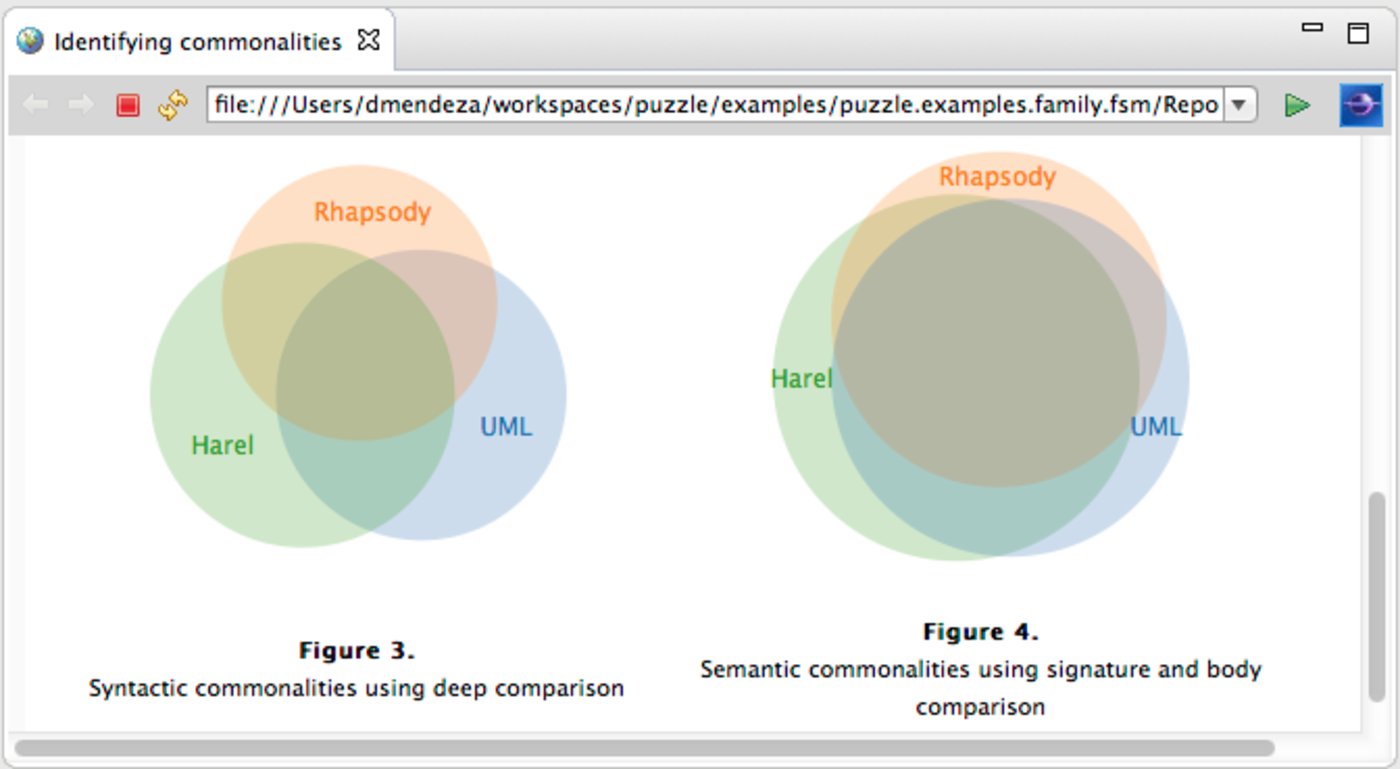
\includegraphics[width=1\linewidth]{images/puzzle-overlapping.pdf}
\caption{Results for the state machines case study: identifying overlapping}
\label{fig:puzzle-overlapping}
\end{figure}

Figure \ref{fig:puzzle-modularization} shows the results for the second and third part of our approach: identifying and extracting reusable language modules. Note that there is a language module (core) that contains all the language constructs that are shared by the three DSLs. Then, the other language modules encapsulate pseudostates and triggers separately since they represent the differences among the DSLs. Note that in order to obtain the Harel's state charts language, we need to compose the modules 1, 2, and 5. In turn, to obtain UML we need to compose modules 1, 3, and 4. Finally, to obtain Rhapsody we need to compose modules 1 and 5.

\begin{figure}
\centering
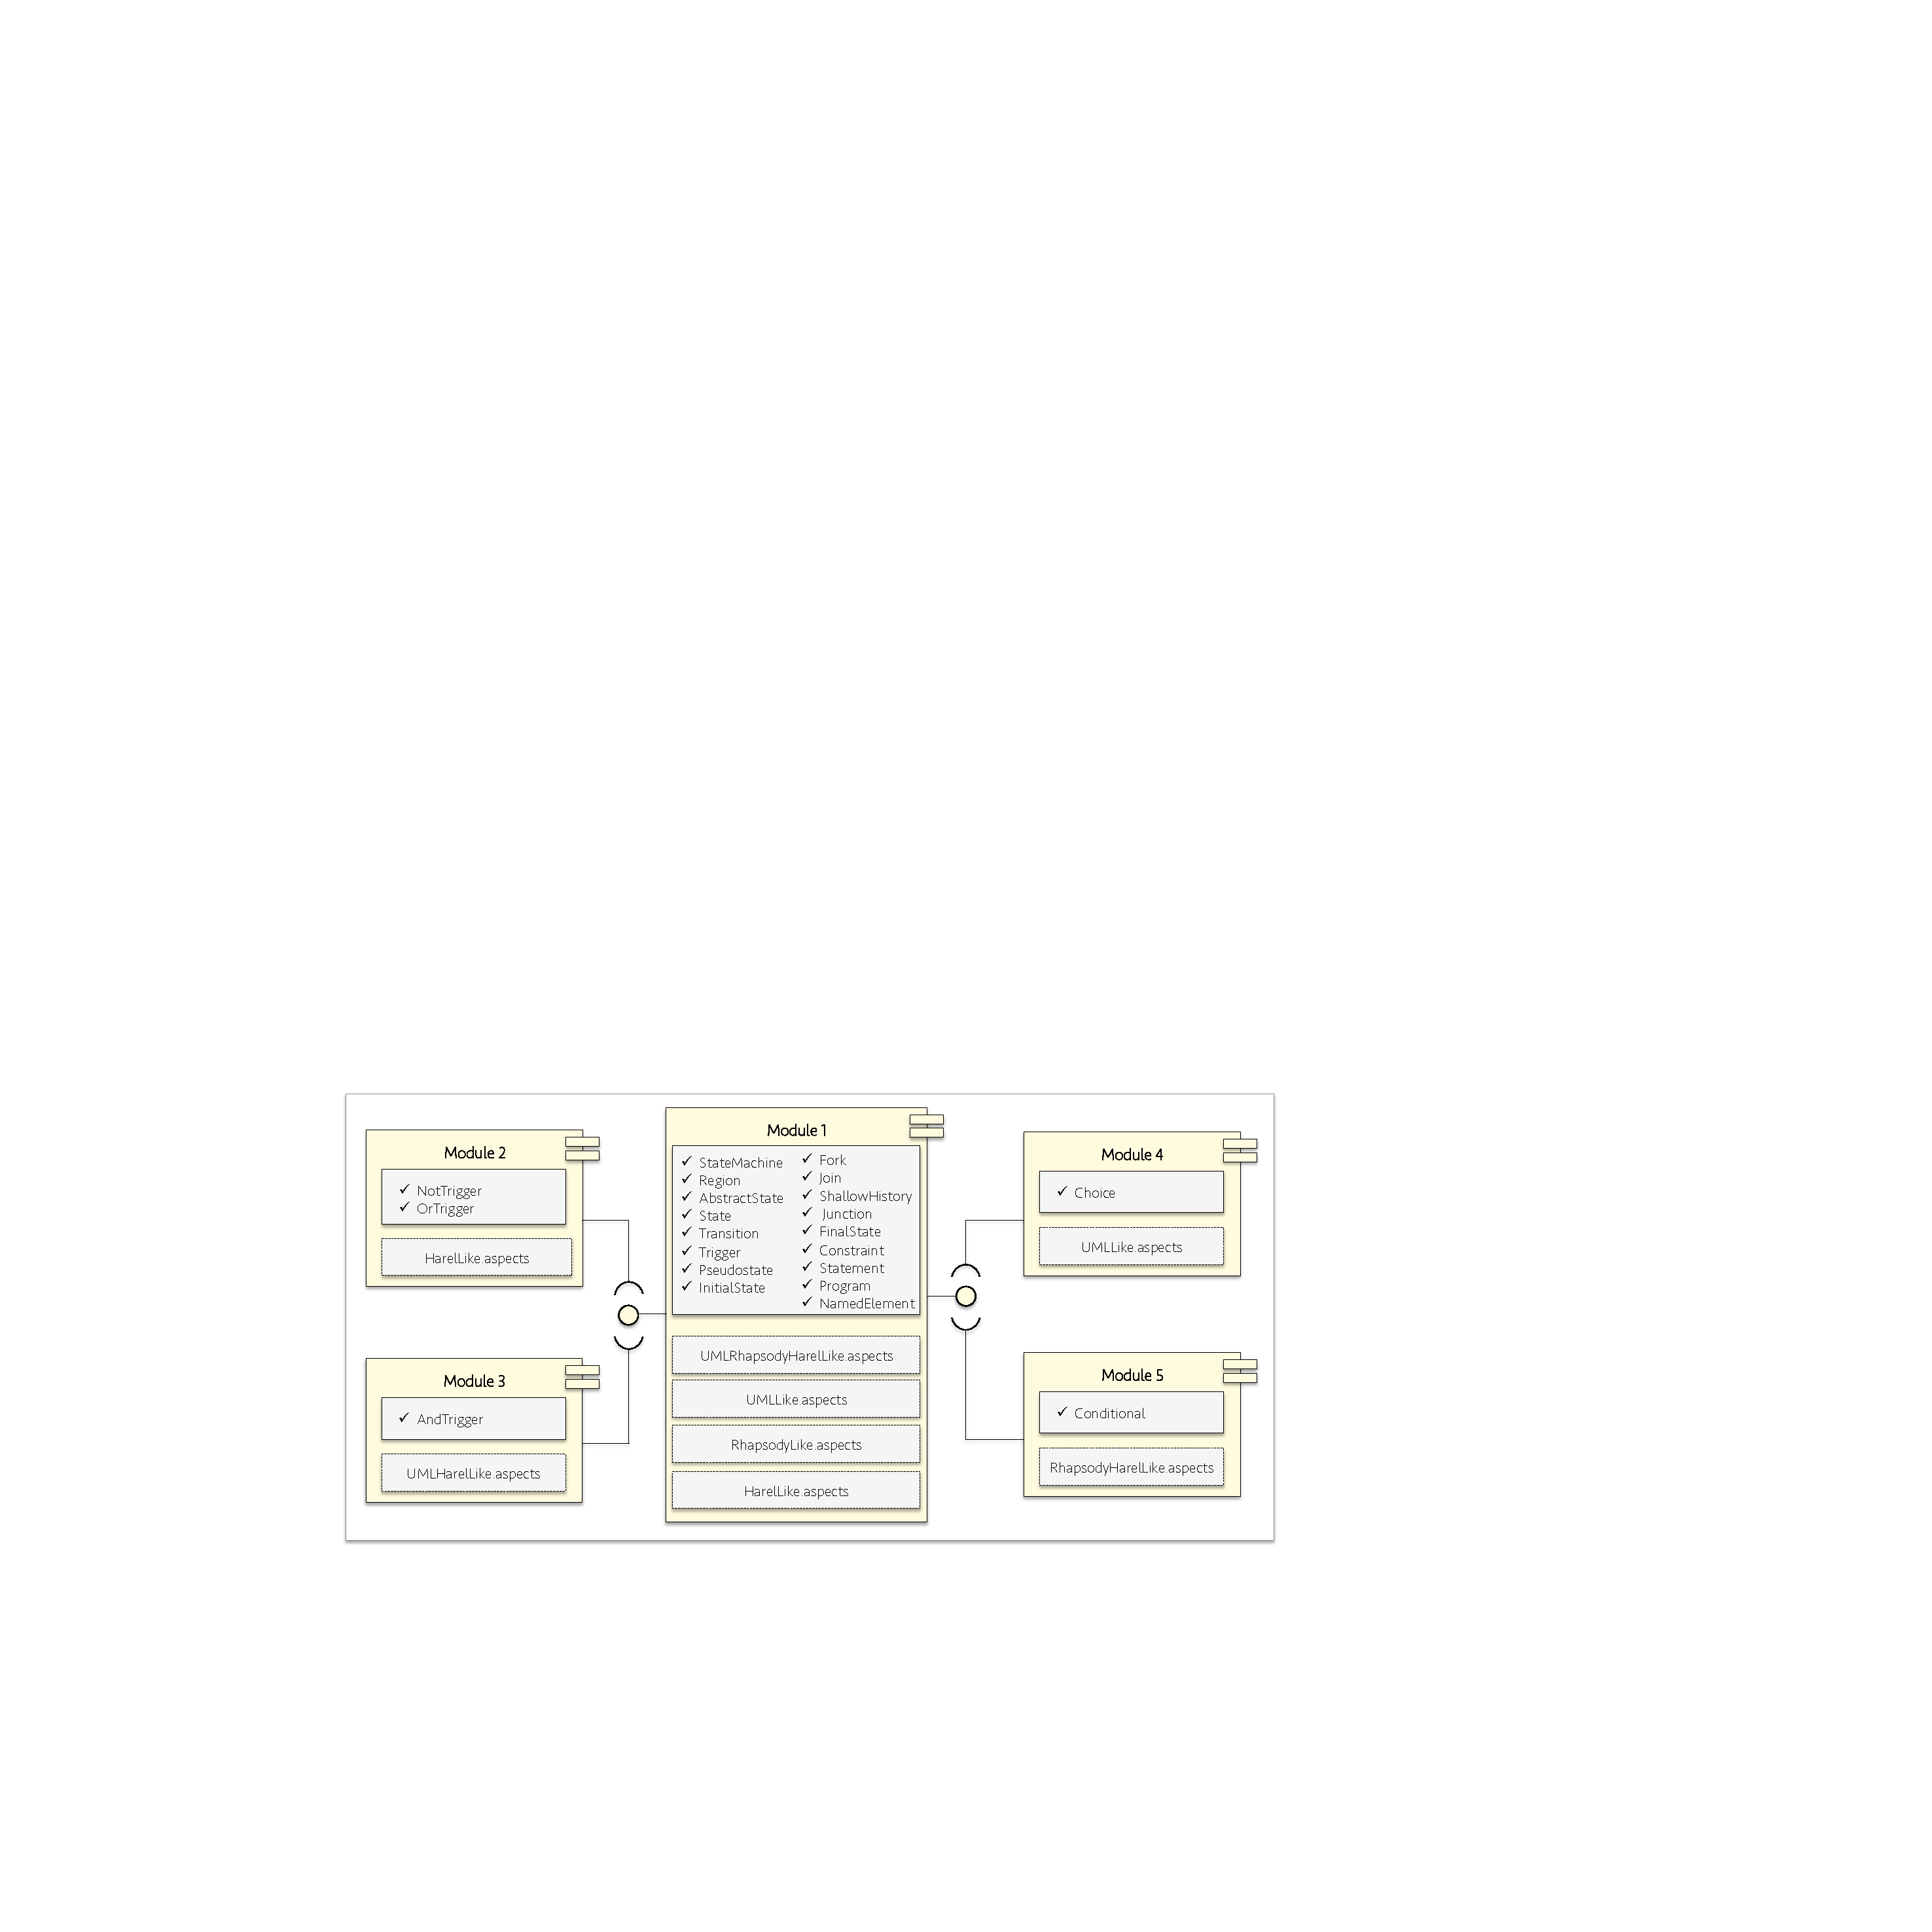
\includegraphics[width=1\linewidth]{images/puzzle-modularization.pdf}
\caption{Results for the state machines case study: extracting language modules}
\label{fig:puzzle-modularization}
\end{figure}

\subsection{Evaluating \textit{relevance}: Identifying potential reuse in the wild}

In order to identify potential reuse in the wild, we explore the public GitHub repositories in searching of DSLs built on the same with the technological space and language workbench that we used in our approach, i.e., metamodels written in Ecore with operational semantics defined in Xtend as domain-specific actions. The objective was to find DSLs developed by diverse development team and with different purposes in order to detect commonalities among them. 

As the result of this exercise, we found an important amount of Ecore metamodels (2800 after discarding metamodels with errors). Contrariwise, due to the fact that Kermeta 3 and its implementation in Xtend is a quite recent idea, we only found some few DSLs. We decided to conduct the approach only in the metamodels. We consider that such analysis a good insight to know if there is potential reuse.

\begin{center}
\textbf{\textit{Experiments under construction...}}
\end{center}

The experiments were conducted using a version of \toolname implemented in Java. Further, 
\toolname was installed in the Grid5000 Cloud, which is a cluster with more than 5000 cores from were we took XX dual-CPU Dell Blades with Intel Xeon X3470 CPUs running at 2.93GHz, with 16 threads 
per CPU, and CentOS v6. Each dual-CPU Dell Blade has 36GB of RAM. 

%\begin{table*}[htbp]
%  \centering
% \scalebox{0.8}{
%\begin{tabular}{|p{0.2\textwidth}|p{0.3\textwidth}p{0.1\textwidth}p{0.4\textwidth}|}
%\hline
%\multicolumn{4}{|c|}{\textbf{Hypotheses of Experiment 1}} \\ \hline
%\textbf{Null Hypothesis ($H_0$)} & \multicolumn{ 3}{|p{0.8\textwidth}|}{\toolname is capable of detecting %commonalities in the case study that motivated this research.} \\ \hline
%\textbf{Alt. Hypothesis ($H_1$)} & \multicolumn{ 3}{|p{0.8\textwidth}|}{
%\toolname is not capable of detecting commonalities in the case study that motivated this research.} \\ %\hline
%\textbf{Dependent variable} & \multicolumn{ 3}{|p{0.8\textwidth}|}{The set of ecores representing our %languages. }\\ \hline
%\textbf{Blocking variables} & \multicolumn{ 3}{|p{0.8\textwidth}|}{The most sold phones and the market %share indexes. }\\ \hline
%\textbf{Model used as input} & \multicolumn{ 3}{|p{0.8\textwidth}|}{\textit{models in %\url{urlhacialosmodelos}} }
%\\
%\hline \hline


%\multicolumn{4}{|c|}{\textbf{Hypotheses of Experiment 2}} \\ \hline
%\textbf{Null Hypothesis ($H_0$)} & \multicolumn{ 3}{|p{0.8\textwidth}|}{The use of \toolname 
%will not result in a higher market-share impact metric than selecting the most commonly sold 
%phones, for a given maximum budget.} \\ \hline
%\textbf{Alt. Hypothesis ($H_1$)} & \multicolumn{ 3}{|p{0.8\textwidth}|}{The use of \toolname 
%will result in a higher market-share impact metric than selecting the most commonly sold 
%phones, for a given maximum budget.}\\ \hline
%\textbf{Model used as input} & \multicolumn{ 3}{|p{0.8\textwidth}|}{\textit{Android feature model presented %in Figure \ref{fig:featureModel}} }\\ 
%\hline
%% @J - Do you mean independent?! My understanding is that a blocking variable is a grouping variable...
%\textbf{Blocking variables} & \multicolumn{ 3}{|p{0.8\textwidth}|}{The most sold phones, market share %indexes and the maximum cost allowed set to 600\$. }\\ \hline
%\textbf{Model used as input} & \multicolumn{ 3}{|p{0.8\textwidth}|}{\textit{Android feature model presented in Figure \ref{fig:featureModel}} }\\
%\hline \hline

%\multicolumn{4}{|c|}{\textbf{Constants}} \\ \hline
%\textbf{CSP solver} & \multicolumn{ 3}{|p{0.8\textwidth}|}{\textit{ChocoSolver v2} } \\ \hline
%\textbf{Heuristic for variable selection in the CSP solver} & \multicolumn{ 3}{|p{0.8\textwidth}|}{\textit{Default}}\\
%\hline 

%\hline 
%\end{tabular}%
%}
%\caption{Hypotheses and design of experiments.}
%  \label{tab:Exp1aDesign}
%\end{table*}
%\todo{poner la tabla para con los datos de los experimentos que vamos a ejecutar/hemos ejecutado. Intenta pensar cuales pueden ser las conclusiones que quieres extraer. Yo propongo 3 abajo.}

%Table \ref{tab:Exp1aDesign} shows the hypothesis of the experiments executed to validate our 
%approach. To make the experiments reproducible, a number of fixed assumptions are made, such as homogeneous feature costs. ChocoSolver 
%\footnote{\url{http://www.emn.fr/z-info/choco-solver/}}, with it's default heuristic, is 
%used as the CSP solver for extracting software products from the feature model presented 
%in Figure \ref{fig:featureModel}

%\textbf{Technological space and experimental platform:} Currently, there are diverse techniques available for the implementation of syntax and semantics of DSLs \cite{Mernik:2005b}. Language designers can, for example, choose between using context-free grammars or metamodels as specification formalism for syntax. Similarly, there are at least three methods for expressing semantics: operationally, denotationally, and axiomatically \cite{Mosses:2001}. In this paper we are interested on DSLs which syntax is specified by means of metamodels and semantics is specified operationally as a set methods (a.k.a, \textit{domain-specific actions} \cite{Combemale:2013}). Each language construct is specified by means a metaclass and the relationship between language constructs are specified as references between metaclasses. In turn, domain-specific actions are specified as java-like methods that are allocated in each metaclass.

%\section{Tool demonstration}
\label{sec:tooldemo}

The approach presented in this paper is tool-supported. That means that we implemented a the tooling needed to support the ideas and concepts. The tooling is implemented on top of Eclipse IDE and, in particular, the Eclipse Modeling Framework. In the following, we present two different videos. The first one illustrates the use of our tool in the illustrating example presented in section \ref{sec:motivation}. The second video shows the tool for the case study of the state machines presented in section \ref{sec:validation}.

\begin{itemize}
\item \textbf{Tool demonstration 1:} FSM, Logo, and Flowcharts. URL: video

\item \textbf{Tool demonstration 2:} UML state diagrams, Rhapsody, and Harel state charts. URL: video
\end{itemize}

%\section{Threads to validity}
\label{sec:threadstovalidity}

The most important thread to validity of our tool corresponds to the constraint that all the members of the family must be implemented in the same technology. We are aware that this constraints limits the applicability of our tool since it is possible to find families of DSLs where each member is implemented in a different tool. However, we have two points to discuss to this regard.

First, the problem we are trying to solve has to be with adaptation of the same DSL. As we mentioned in the introduction, one of the situations where families of DSLs appear is where an initial language is adapted for fit a particular domain. Under this situation, we can expect that the technologies are the same. 

Second, the contribution of this paper is not only limited to the tool itself. All the ideas expressed here with respect to the issues that are important to analyze in a family of DSLs are important as well. We consider that our tool can be conceived for other technologies. 
%\section{Related work and discussion}
\label{sec:relatedwork}

Leveraging reuse in the construction of DSLs is an objective that has been previously discussed in the research community on software languages engineering. One of the very first achievements towards this objective was the notion of components-based language development. With the time passing, approaches are becoming more sophisticate, thus supporting more complex modularization scenarios, and being applicable for more diverse technological spaces \cite{Mernik:2013,Rumpe:2010,Voelter:2013b}. 

More recent approaches are focused not only on dealing with modularization issues, but also on facilitating the reuse process itself. For instance, Melange \cite{Degueule:2015} is a tool-supported approach that introduces some operators (such as slice, inheritance, and merge) intended to manipulate legacy DSLs in such a way that they can be easily integrated in new developments. Using Melange, a language designer can combine a set of DSLs in different ways to produce a new one.

The main contribution of our approach is that it advances towards the automation of the reuse process. We demonstrate that, with the correct abstractions and assuming some constraints, the process can be automated by means of reverse-engineering techniques. It is important mentioning that our approach uses some of the ideas presented by Caldiera and Basili \cite{Caldiera:1991}. That approach proposes reverse-engineering methodologies for extracting reusable modules in objects oriented software. In addition, our work is based on an observation about commonalities and potential reuse provided by V\"oelter et al \cite[p. 60-61]{voelter:2013}. We show that the notion of commonalities is quite useful for extracting reusable language modules.

There are, however, some open issues that need further investigation. In particular, during the conduction of this research, and trying to apply the approach in further case studies, we realized that the comparison operators to detect those commonalities can become an Achilles' heel. In some cases, the notion of commonality can be associated to a given \textit{functionality} (abstractly speaking), more than equality in the specification. For example, there are many DSLs that use constraints languages but that use different language constructs to support them. They share the functionality of constraint languages, but the specifications do not match. That does not mean that there is not potential reuse. The detection of this kind of commonalities can become quite difficult due to the ambiguity in that notion of functionality.

As a matter of fact, considering more flexible approaches for the detection of commonalities can have additional advantages. Consider for example two DSL that define different constraints languages where one is better defined (more completely or with more powerful capabilities) than the other. If this situations can be detected, and language designers can chose a preferred language module, our approach can become useful not only to achieve reuse but also to improve quality of existing DSLs. We claim that more complex overlapping identification (probably with human intervention) should be provided.

%Software reuse has been largely studied during the last decades. The complexity behind the definition of reusable software is well-known and many approaches has been proposed to facilitate this task. The work of Caldiera and Basili \cite{Caldiera:1991} is a clear example of such approaches. It is intended to automatically extract reusable software modules from existing software systems. Then, a set of metrics for qualifying the quality of the produced modules. As mentioned in the introduction, this work has inspired the approach presented in that work paper. 

%The main contribution of the research presented this paper is that we apply those ideas in the construction of DSLs. To do so, we use a strategy based on Venn diagrams that, in turn, has been inspired in the phenomenon of domains overlapping identified by .

%As a matter of fact, our approach is not the first one that tries to increase reuse in the construction of DSLs. The community of software languages engineering has been intensively working on this issue and noways we can find approaches for components-based languages development (such as ). In that context, our approach can be positioned as a reverse engineering technique for increasing reuse where reusable language modules are extracted from existing DSLs. It is worth noting that there are other approaches working on reverse engineering for DSLs. For example, the research presented in \cite{vacchi:2014} and \cite{Kuhn:2015}, is intended to synthesize language product lines (i.e., software product lines where the products are DSLs) from a DSL specification. 

 


%\section{Conclusions and future work}
\label{sec:conclusions}
%lessons learned????
%\todo[inline]{eventualmente tenemos que extender esta parte... aunque no hay mucho sitio... escribela si peudes y ya vemos que hacemos... si no para la extension de revista ;)}
In this paper, we presented an approach to exploit reuse during the construction of DSLs. We show that it is possible to partially automate the reuse process by identifying overlapping among DSLs and automatically extracting reusable language modules that can be later used in the construction of new DSLs.

We evaluated our approach in a real industrial case study and we demonstrate that there is an important amount of potential reuse in DSLs in public repositories. More concretely, based on empirical data, we showed that in about the \textbf{40\%} of the new DSLs there are reuse opportunities to exploit reuse. This reuse is, in average, about the \textbf{10\%} of the size of the DSLs. 

As future work, we plan to propose approaches to automatically build language product lines i.e., software product lines where the products are DSLs. The intention is to follow with the idea of automating the reuse process. This time, using ideas that facilitate the management of the variability existing among DSLs. 

\section*{Acknowledgments}
The research presented in this paper is supported by the European Union within the FP7 Marie Curie Initial Training Network ``RELATE" under grant agreement number 264840 and VaryMDE, a collaboration between Thales and INRIA.

% BIBLIOGRAPHY
\bibliographystyle{abbrv}
\bibliography{0-main}

\end{document}
